%%%%%%%%%%%%%%%%%%%%
%%% Document
%%%%%%%%%%%%%%%%%%%%
\documentclass[pdftex, a4paper,11pt, twoside, ngerman]{report}
% \documentclass[11pt,xcolor=dvipsnames]{beamer}

% für deutsche zeichen äüö ohne kile auto-ersetzen
% \usepackage[utf8x]{inputenc}

% kile auto-ersetzen: einstellungen->latex:general-> hacken bei special
% characters
% \usepackage[ansinew]{inputenc}
% \usepackage[UKenglish]{babel}          %Englisch
\usepackage[ngerman]{babel}          %Deutsch


%%%%%%%%%%
%%% Geometry
%%%%%%%%%%
% \usepackage{showframe}
\usepackage[scale=0.8, hmarginratio=4:2]{geometry}
\geometry{%
  textheight     = 1.05\textheight,
  textwidth      = 0.95\textwidth,
  headheight     = 15 pt,
  %       footheight     = 15 pt,
  marginparwidth = 82 pt}
\parskip=7pt
\renewcommand{\arraystretch}{1.2}
% \pagestyle{fancy}



%%%%%%%%%%
%%% Packages (aus header datei)
%%%%%%%%%%
\IfFileExists{header_TobiasBrauell-DOCUMENT.tex}{
    % Copyright © 2014 Tobias Brauell <tobiasbrauell@gmail.com>

% This is my general purpose LaTeX header file for writing German documents.
% Ideally, you include this using a simple ``\input{header.tex}`` in your main
% document and start with ``\title`` and ``\begin{document}`` afterwards.

% If you need to add additional packages, I recommend not doing this in this
% file, but in your main document. That way, you can just drop in a new
% ``header.tex`` and get all the new commands without having to merge manually.

%%%%%%%%%%%%%%%%%%%%%%%%%%%%%
%%% Locale, date
%%%%%%%%%%%%%%%%%%%%%%%%%%%%%
\usepackage[UKenglish]{isodate}



%%%%%%%%%%%%%%%%%%%%%%%%%%%%%
%%% Margins and other spacing
%%%%%%%%%%%%%%%%%%%%%%%%%%%%%
\usepackage[activate]{pdfcprot}
% \usepackage[parfill]{parskip}
\usepackage{setspace}
  \setlength{\columnsep}{2 cm}
  \setlength{\parindent}{0 pt}


%%%%%%%%%%%%%%%%%%%%%%%%%%%%%
%%% Input encoding
%%%%%%%%%%%%%%%%%%%%%%%%%%%%%
\usepackage[T1]{fontenc}
\usepackage[utf8x]{inputenc}



%%%%%%%%%%%%%%%%%%%%%%%%%%%%%
%%% Indexing
%%%%%%%%%%%%%%%%%%%%%%%%%%%%%
\usepackage{makeidx}
  \makeindex



%%%%%%%%%%%%%%%%%%%%%%%%%%%%%
%%% Blindtext
%%%%%%%%%%%%%%%%%%%%%%%%%%%%%
\usepackage{blindtext}


%%%%%%%%%%%%%%%%%%%%%%%%%%%%%
%%% Global Counter
%%%%%%%%%%%%%%%%%%%%%%%%%%%%%



%%%%%%%%%%%%%%%%%%%%%%%%%%%%%
%%% Geometry
%%%%%%%%%%%%%%%%%%%%%%%%%%%%%
\usepackage{layout}
% \usepackage[scale=0.8]{geometry}
%   \geometry{textheight=1.05\textheight, marginparwidth=50 pt}

% \usepackage{multirow}
% \usepackage{dcolumn}



%%%%%%%%%%%%%%%%%%%%%%%%%%%%%
%%% Pagestyle
%%%%%%%%%%%%%%%%%%%%%%%%%%%%%
% \usepackage{fancyhdr}
% \usepackage{microtype} 

% \pagestyle{fancy}



%%%%%%%%%%%%%%%%%%%%%%%%%%%%%
%%% Fonts/Colors
%%%%%%%%%%%%%%%%%%%%%%%%%%%%%
\usepackage{lmodern}
\usepackage{xcolor}
% This replaces all fonts with Bitstream Charter, Bitstream Vera Sans and
% Bitstream Vera Mono. Math will be rendered in Charter.
% \usepackage[charter, greekuppercase=italicized]{mathdesign}
% \usepackage{beramono}
% \usepackage{berasans}

% Bold, sans-serif tensors. This fragment is taken from “egreg” from
% http://tex.stackexchange.com/a/82747/8945 and licensed under `CC-BY-SA
% <https://creativecommons.org/licenses/by-sa/3.0/>`_.
% \usepackage{bm}
%   \DeclareMathAlphabet{\mathsfit}{\encodingdefault}{\sfdefault}{m}{sl}
%   \SetMathAlphabet{\mathsfit}{bold}{\encodingdefault}{\sfdefault}{bx}{sl}
%   \newcommand{\tens}[1]{\bm{\mathsfit{#1}}}

% Bold vectors.
% \renewcommand{\vec}[1]{\boldsymbol{#1}}



%%%%%%%%%%%%%%%%%%%%%%%%%%%%%
%%% Code/Listings
%%%%%%%%%%%%%%%%%%%%%%%%%%%%%
\usepackage{listings}



%%%%%%%%%%%%%%%%%%%%%%%%%%%%%
%%% Enumerations
%%%%%%%%%%%%%%%%%%%%%%%%%%%%%
\usepackage{enumitem}
% \usepackage{paralist}


%%%%%%%%%%%%%%%%%%%%%%%%%%%%%
%%% Figures
%%%%%%%%%%%%%%%%%%%%%%%%%%%%%
% \usepackage[pdftex]{graphicx}
\usepackage{graphicx}
\usepackage{epsfig}
\usepackage{epstopdf}
\usepackage{subfigure}
\usepackage{wrapfig}
\makeatletter \newcommand\hyper@makecurrent[1]{} \makeatother
\usepackage{caption}
% \usepackage{subcaption}

\addto\captionsUKenglish{\renewcommand{\figurename}{Fig.}}
\addto\captionsngerman{\renewcommand{\figurename}{Abb.}}



%%%%%%%%%%%%%%%%%%%%%%%%%%%%%
%%% PDF Pages
%%%%%%%%%%%%%%%%%%%%%%%%%%%%%
\usepackage{pdfpages}



%%%%%%%%%%%%%%%%%%%%%%%%%%%%%
%%% Personal Graphics
%%%%%%%%%%%%%%%%%%%%%%%%%%%%%
\usepackage{tikz}
% \usepackage{tikz-3dplot}
  \usetikzlibrary{calc}
  \usetikzlibrary{decorations.markings}



%%%%%%%%%%%%%%%%%%%%%%%%%%%%%
%%% Math
%%%%%%%%%%%%%%%%%%%%%%%%%%%%%
\usepackage{amsmath}
\usepackage{amssymb}
\usepackage{mathtools}
\usepackage{dcolumn}
\usepackage{siunitx}
% \usepackage{feynmf}



%%%%%%%%%%%%%%%%%%%%%%%%%%%%%
%%% Referenzen
%%%%%%%%%%%%%%%%%%%%%%%%%%%%%
\usepackage{hyperref}
\usepackage{url}
% \usepackage{cleveref}%\label{abc}--\cref{abc} \Cref{abc[,def]}-und \crefrange{abc}{def}-bis
\usepackage[english]{cleveref}%\label{abc}--\cref{abc} \Cref{abc[,def]}-und \crefrange{abc}{def}-bis



%%%%%%%%%%%%%%%%%%%%%%%%%%%%%
%%% Table's
%%%%%%%%%%%%%%%%%%%%%%%%%%%%%
\usepackage{rotating}
\usepackage{longtable}
\usepackage{multirow}
\usepackage{tabularx}
  \newcolumntype{L}[1]{>{\raggedright\arraybackslash}p{#1}} % linksbündig mit Breitenangabe
  \newcolumntype{C}[1]{>{\centering\arraybackslash}p{#1}} % zentriert mit Breitenangabe
  \newcolumntype{R}[1]{>{\raggedleft\arraybackslash}p{#1}} % rechtsbündig mit Breitenangabe



%%%%%%%%%%%%%%%%%%%%%%%%%%%%%
%%% Todo's
%%%%%%%%%%%%%%%%%%%%%%%%%%%%%
% \usepackage{xkeyval}
\usepackage{todonotes} %\todo{text} oder \todo[inline]{text}
%   \presetkeys{todonotes}{inline}{}
%   \let\todox\todo
%   \renewcommand\todo{1}{\todox[inline]{#1}}


%%%%%%%%%%%%%%%%%%%%%%%%%%%%%%%%%%%%%%%%%%%%%%%%%%%%%%%%%%
%%% Settings
%%%%%%%%%%%%%%%%%%%%%%%%%%%%%%%%%%%%%%%%%%%%%%%%%%%%%%%%%%
\usepackage{cancel}

\newcommand{\HRule}{\rule{\linewidth}{0.5mm}}



%%%%%%%%%%%%%%%%%%%%%%%%%%%%%
%%% Theme
%%%%%%%%%%%%%%%%%%%%%%%%%%%%%



%%%%%%%%%%%%%%%%%%%%%%%%%%%%%
%%% header
%%%%%%%%%%%%%%%%%%%%%%%%%%%%%
% \lhead{text}
% \chead{text}
% \rhead{text}



%%%%%%%%%%%%%%%%%%%%%%%%%%%%%
%%% footer
%%%%%%%%%%%%%%%%%%%%%%%%%%%%%
%%% Tobias Brauell       	Versuch....		Ruth Jacobs
% \renewcommand\footrulewidth{.4pt}
% \lfoot{\scriptsize Ruth Jacobs - Tobias Brauell \\ {\ \ \ \ \ \ \ \ \ \ } Gruppe $\alpha 9$} 
% \cfoot{\thepage\ / \ \pageref{LastPage}}
% \rfoot{\scriptsize Versuch 518: Höhenstrahlung \\ Tutor: Christoph Krieger {\ \ \ } } 



%%%%%%%%%%%%%%%%%%%%%%%%%%%%%
%%% Title Page
%%%%%%%%%%%%%%%%%%%%%%%%%%%%%
% \title[ITER { } International Thermonuclear Experimental Reactor]{\huge{\bf{ITER}} \\ \large{\bf{International Thermonuclear Experimental Reactor}}}
% \author[T. Brauell]{Tobias Brauell}
% \institute{Universität Bonn}
% 
% \date{09.~Dez.~2013}
% \logo{\includegraphics[width=.15\textwidth]{Figures/toplogo.png}}


}{
    % Copyright © 2014 Tobias Brauell <tobiasbrauell@gmail.com>

% This is my general purpose LaTeX header file for writing German documents.
% Ideally, you include this using a simple ``\input{header.tex}`` in your main
% document and start with ``\title`` and ``\begin{document}`` afterwards.

% If you need to add additional packages, I recommend not doing this in this
% file, but in your main document. That way, you can just drop in a new
% ``header.tex`` and get all the new commands without having to merge manually.

%%%%%%%%%%%%%%%%%%%%%%%%%%%%%
%%% Locale, date
%%%%%%%%%%%%%%%%%%%%%%%%%%%%%
\usepackage[UKenglish]{isodate}



%%%%%%%%%%%%%%%%%%%%%%%%%%%%%
%%% Margins and other spacing
%%%%%%%%%%%%%%%%%%%%%%%%%%%%%
\usepackage[activate]{pdfcprot}
% \usepackage[parfill]{parskip}
\usepackage{setspace}
  \setlength{\columnsep}{2 cm}
  \setlength{\parindent}{0 pt}


%%%%%%%%%%%%%%%%%%%%%%%%%%%%%
%%% Input encoding
%%%%%%%%%%%%%%%%%%%%%%%%%%%%%
\usepackage[T1]{fontenc}
\usepackage[utf8x]{inputenc}



%%%%%%%%%%%%%%%%%%%%%%%%%%%%%
%%% Indexing
%%%%%%%%%%%%%%%%%%%%%%%%%%%%%
\usepackage{makeidx}
  \makeindex



%%%%%%%%%%%%%%%%%%%%%%%%%%%%%
%%% Blindtext
%%%%%%%%%%%%%%%%%%%%%%%%%%%%%
\usepackage{blindtext}


%%%%%%%%%%%%%%%%%%%%%%%%%%%%%
%%% Global Counter
%%%%%%%%%%%%%%%%%%%%%%%%%%%%%



%%%%%%%%%%%%%%%%%%%%%%%%%%%%%
%%% Geometry
%%%%%%%%%%%%%%%%%%%%%%%%%%%%%
\usepackage{layout}
% \usepackage[scale=0.8]{geometry}
%   \geometry{textheight=1.05\textheight, marginparwidth=50 pt}

% \usepackage{multirow}
% \usepackage{dcolumn}



%%%%%%%%%%%%%%%%%%%%%%%%%%%%%
%%% Pagestyle
%%%%%%%%%%%%%%%%%%%%%%%%%%%%%
% \usepackage{fancyhdr}
% \usepackage{microtype} 

% \pagestyle{fancy}



%%%%%%%%%%%%%%%%%%%%%%%%%%%%%
%%% Fonts/Colors
%%%%%%%%%%%%%%%%%%%%%%%%%%%%%
\usepackage{lmodern}
\usepackage{xcolor}
% This replaces all fonts with Bitstream Charter, Bitstream Vera Sans and
% Bitstream Vera Mono. Math will be rendered in Charter.
% \usepackage[charter, greekuppercase=italicized]{mathdesign}
% \usepackage{beramono}
% \usepackage{berasans}

% Bold, sans-serif tensors. This fragment is taken from “egreg” from
% http://tex.stackexchange.com/a/82747/8945 and licensed under `CC-BY-SA
% <https://creativecommons.org/licenses/by-sa/3.0/>`_.
% \usepackage{bm}
%   \DeclareMathAlphabet{\mathsfit}{\encodingdefault}{\sfdefault}{m}{sl}
%   \SetMathAlphabet{\mathsfit}{bold}{\encodingdefault}{\sfdefault}{bx}{sl}
%   \newcommand{\tens}[1]{\bm{\mathsfit{#1}}}

% Bold vectors.
% \renewcommand{\vec}[1]{\boldsymbol{#1}}



%%%%%%%%%%%%%%%%%%%%%%%%%%%%%
%%% Code/Listings
%%%%%%%%%%%%%%%%%%%%%%%%%%%%%
\usepackage{listings}



%%%%%%%%%%%%%%%%%%%%%%%%%%%%%
%%% Enumerations
%%%%%%%%%%%%%%%%%%%%%%%%%%%%%
\usepackage{enumitem}
% \usepackage{paralist}


%%%%%%%%%%%%%%%%%%%%%%%%%%%%%
%%% Figures
%%%%%%%%%%%%%%%%%%%%%%%%%%%%%
% \usepackage[pdftex]{graphicx}
\usepackage{graphicx}
\usepackage{epsfig}
\usepackage{epstopdf}
\usepackage{subfigure}
\usepackage{wrapfig}
\makeatletter \newcommand\hyper@makecurrent[1]{} \makeatother
\usepackage{caption}
% \usepackage{subcaption}

\addto\captionsUKenglish{\renewcommand{\figurename}{Fig.}}
\addto\captionsngerman{\renewcommand{\figurename}{Abb.}}



%%%%%%%%%%%%%%%%%%%%%%%%%%%%%
%%% PDF Pages
%%%%%%%%%%%%%%%%%%%%%%%%%%%%%
\usepackage{pdfpages}



%%%%%%%%%%%%%%%%%%%%%%%%%%%%%
%%% Personal Graphics
%%%%%%%%%%%%%%%%%%%%%%%%%%%%%
\usepackage{tikz}
% \usepackage{tikz-3dplot}
  \usetikzlibrary{calc}
  \usetikzlibrary{decorations.markings}



%%%%%%%%%%%%%%%%%%%%%%%%%%%%%
%%% Math
%%%%%%%%%%%%%%%%%%%%%%%%%%%%%
\usepackage{amsmath}
\usepackage{amssymb}
\usepackage{mathtools}
\usepackage{dcolumn}
\usepackage{siunitx}
% \usepackage{feynmf}



%%%%%%%%%%%%%%%%%%%%%%%%%%%%%
%%% Referenzen
%%%%%%%%%%%%%%%%%%%%%%%%%%%%%
\usepackage{hyperref}
\usepackage{url}
% \usepackage{cleveref}%\label{abc}--\cref{abc} \Cref{abc[,def]}-und \crefrange{abc}{def}-bis
\usepackage[english]{cleveref}%\label{abc}--\cref{abc} \Cref{abc[,def]}-und \crefrange{abc}{def}-bis



%%%%%%%%%%%%%%%%%%%%%%%%%%%%%
%%% Table's
%%%%%%%%%%%%%%%%%%%%%%%%%%%%%
\usepackage{rotating}
\usepackage{longtable}
\usepackage{multirow}
\usepackage{tabularx}
  \newcolumntype{L}[1]{>{\raggedright\arraybackslash}p{#1}} % linksbündig mit Breitenangabe
  \newcolumntype{C}[1]{>{\centering\arraybackslash}p{#1}} % zentriert mit Breitenangabe
  \newcolumntype{R}[1]{>{\raggedleft\arraybackslash}p{#1}} % rechtsbündig mit Breitenangabe



%%%%%%%%%%%%%%%%%%%%%%%%%%%%%
%%% Todo's
%%%%%%%%%%%%%%%%%%%%%%%%%%%%%
% \usepackage{xkeyval}
\usepackage{todonotes} %\todo{text} oder \todo[inline]{text}
%   \presetkeys{todonotes}{inline}{}
%   \let\todox\todo
%   \renewcommand\todo{1}{\todox[inline]{#1}}


%%%%%%%%%%%%%%%%%%%%%%%%%%%%%%%%%%%%%%%%%%%%%%%%%%%%%%%%%%
%%% Settings
%%%%%%%%%%%%%%%%%%%%%%%%%%%%%%%%%%%%%%%%%%%%%%%%%%%%%%%%%%
\usepackage{cancel}

\newcommand{\HRule}{\rule{\linewidth}{0.5mm}}



%%%%%%%%%%%%%%%%%%%%%%%%%%%%%
%%% Theme
%%%%%%%%%%%%%%%%%%%%%%%%%%%%%



%%%%%%%%%%%%%%%%%%%%%%%%%%%%%
%%% header
%%%%%%%%%%%%%%%%%%%%%%%%%%%%%
% \lhead{text}
% \chead{text}
% \rhead{text}



%%%%%%%%%%%%%%%%%%%%%%%%%%%%%
%%% footer
%%%%%%%%%%%%%%%%%%%%%%%%%%%%%
%%% Tobias Brauell       	Versuch....		Ruth Jacobs
% \renewcommand\footrulewidth{.4pt}
% \lfoot{\scriptsize Ruth Jacobs - Tobias Brauell \\ {\ \ \ \ \ \ \ \ \ \ } Gruppe $\alpha 9$} 
% \cfoot{\thepage\ / \ \pageref{LastPage}}
% \rfoot{\scriptsize Versuch 518: Höhenstrahlung \\ Tutor: Christoph Krieger {\ \ \ } } 



%%%%%%%%%%%%%%%%%%%%%%%%%%%%%
%%% Title Page
%%%%%%%%%%%%%%%%%%%%%%%%%%%%%
% \title[ITER { } International Thermonuclear Experimental Reactor]{\huge{\bf{ITER}} \\ \large{\bf{International Thermonuclear Experimental Reactor}}}
% \author[T. Brauell]{Tobias Brauell}
% \institute{Universität Bonn}
% 
% \date{09.~Dez.~2013}
% \logo{\includegraphics[width=.15\textwidth]{Figures/toplogo.png}}


}



%%%%%%%%%%
%%%%%%%%%%
%%%%%%%%%%
\begin{document}
%   \layout
  
  
  
  %%%%%%%%%%%%%%%%%%%%
  %%%%%%%%%%%%%%%%%%%%
  %%%%%%%%%%%%%%%%%%%%
  %%%%%%%%%%%%%%%%%%%%%%%%%%%%%%%%%%%%%%%%%%%%%%%%%%%%%%%%%%
%%% Title Page - Bachelor Thesis
%%%%%%%%%%%%%%%%%%%%%%%%%%%%%%%%%%%%%%%%%%%%%%%%%%%%%%%%%%
\begin{titlepage}
  \thispagestyle{empty}
  \begin{center}

    % Upper part of the page. The '~' is needed because \\
    % only works if a paragraph has started.
%     \includegraphics[width=0.15\textwidth]{./logo}~\\[1cm]
    \begin{minipage}{0.5\textwidth}
      \begin{flushleft}
	
\includegraphics[width=.5\textwidth]{Figures/Logos/logoUNI.png}
      \end{flushleft}
    \end{minipage}%
    \begin{minipage}{0.5\textwidth}
      \begin{flushright}
	
\includegraphics[width=.5\textwidth]{Figures/Logos/logoPI.png}
      \end{flushright}
    \end{minipage}
    
    \vspace{25 pt}
    
    \textsc{\LARGE Rheinische Friedrich-Wilhelms-Universität Bonn}\\[1.5 cm]
    
    \vspace{50 pt}
    
    \textsc{\Large Praktikum 4 - Atome und Moleküle}\\[0.5 cm]

    % Title
    \HRule \\[0.4 cm]
    { \huge \bfseries Versuch 443 - Kernmagnetische Relaxation \\[0.4 cm] }

    \HRule \\[1.5 cm]

    % Author and supervisor
    \noindent
    \begin{minipage}{0.4\textwidth}
      \begin{flushleft} \large
	\emph{Authors:}\\
	Tobias \textsc{Brauell}\\
	Frederike \textsc{Schrödel}
      \end{flushleft}
    \end{minipage}%
    \begin{minipage}{0.4\textwidth}
      \begin{flushright} \large
	\emph{Supervisors:} \\
        Marcel \textsc{Bornstein} \\
        Scott \textsc{Reeve}
      \end{flushright}
    \end{minipage}

    \vfill

    % Bottom of the page
    \HRule \\[0.4 cm]
    {\large \today}

  \end{center}
\end{titlepage}
  %%%%%%%%%%%%%%%%%%%%
  
  
  
%   \setcounter{page}{2}
  
  \begin{chapter}*{Abstract}
    Ziel des Versuchs ist es kernmagnetische Resonanzen zu untersuchen und dabei wichtige Kenngrößen wie die Gitter- und Spin-Spin Relaxationszeiten zu bestimmen.
    Hierzu werden Protonen, in Form von Wasserstoff in leichtem Mineralöl, in einem magnetischen Wechselfeld angeregt und die daraus resultierende Magnetisierung beobachtet.
    
    \todo[inline]{TO-DO}
    
  \end{chapter}
  
  \tableofcontents
  
  
  
  %%%%%%%%%%%%%%%%%%%%
  %%%%%%%%%%%%%%%%%%%%
  %%%%%%%%%%%%%%%%%%%%
  \begin{chapter}{Theorie des Versuchs}
    \label{chp:Theorie}
    
    \begin{section}{Protonen im homogene Magnetfeld}
        In diesen Versuch experementieren wir mit Probe, welche Protonen bereitstellt.
        Protonen haben einen Spin $ s = \frac 12$ mit einer z-Komponente $m_s = -\frac 12 , \frac 12$.
        Aufgrund des Spins besitzen Protonen ein magnetisches Moment $\mu$, welches parallel zum Spin steht.
        \[
            \mu = \gamma\hbar s
        \]
        Wobei $\gamma$ das gyromagnetische Verhältnis ist und von der Art des Teilchens abhängig ist.
        Das magnetisch Moment bewirkt im externen Magnetfeld $\vec B$ ein Drehmoment $\vec M$ auf das Proton:
        \[
            \vec M = \vec \mu \times \vec B
        \]
        Darauf hin kommt es zu einer Präzession des mangetischen Moments, in unseren Fall um die z-Achse, wobei die Frequenz gegeben ist durch die sogenannte Lamorfrequenz 
        \[
            \omega_L = \gamma B_z
        \]

        Das Drehmoment führt außerdem zu einer Einestellenergie:
        \[
            E = -\langle \mu ,B_z\rangle
        \]
        Man erhält zwei Zustände \todo{spin up down}, da $m_s$ nur zwei Werte annehmen kann.
        So kommt es durch die Einstellenergie zu zwei unterschiedlichen Energieniveaus, welche ohne externes Feld entartet wären.
        \todo{bild}

    \end{section}
    
    \begin{section}{Thermisches Gleichgewicht}

        In dem Fall, dass das externe Magnetfeld abgestellt ist, befinden sich die Spins in einem beliebigen Zustand.
        Somit liegt keine Magnetisierung vor.

        Besteht allerdings ein Magnetfeld, so bildet sich ein anderes thermisches Gleichgewicht aus, wobei $N_+>N_-$, da sich mehr Protonen im unteren Energiniveau befinden.
        Der Besatzungszahlunterschied ist zwar recht gering, (\todo{begrúndung}), erzeugt dennoch eine makroskopische Magnetisierung entlang der z-Achse.
        Um diesen Besetzungszahlunterschied zu erreichen muss das System, für das im unmagnetisierten Zustand $N_+=N_-$ gilt, die Energie die bei der Erniedrigung der Spins frei wird an die Umgebung, das sogenannte Gitter, abgeben.
        Die Boltzmanverteilung gibt das Verhältnis zwischen $N_-$ und $N_+$ an:
        \[
            \frac{N_-}{N_+} = \mathrm e^{\frac{\Delta U}{k_\text BT}}
        \]
        Die Magnetisierung in Z-Richtung ergibt sich aus:
        \[
            M_Z = (N_+-N_-)\mu
        \]
        und für die Magnetisierung im thermischen Gleichgewicht erhält man
        \[
            M_0 \approx N\frac{\mu^2B}{k_\text BT}
        \]
        mit $N=N_-+N_+$.

    \end{section}

    \begin{section}{Longitudinale Relaxation}

        Um die Magnetisierung zu beschreiben, kann man die Differentialgleichung \todo
       % \[
        %    \dod{M_Z(t)}{t} = \frac{M_0-M_Z}{T_1}
        %\]
        mit der Randbedingung $M_{Z(0)} =0$ lösen und erhält die Zeitentwicklung:
        \[
            M(t) = M_0\big (1-\mathrm e^{-\frac tT_1}\big)
        \]
        Hierbei ist $T_1$ die Spin-Gitter-Relaxationszeit, welche beschreibt, wie lange der Prozess der Magnetisierung, beziehungsweise das zurück drehen der Spins in die Ausgangslage nach abschalten des externen Magnetfeldes dauert.

    \end{section}

    \begin{section}{Bei zusätzlichen Gepulst Feld}
        Zusätzlich zu dem homogenen Feld in Z-Richtung nutzen wir im Verlauf des Versuches noch ein gepulstet Magnetfeld, welches sich in der X-Y-Ebene befindet.

        \begin{subsection}{Blochkugel}
            Um sich das Zwei-Niveau-System der Spins im externen Magnetfeld vor zu stellen, bietet sich die Darstellung als Blochkugel an.
            Die Spins stellen hierbei die Vektoren dar, die auf eine Einheitskugel zeigen.
            Dabei wird der Spin up durch den Vektor (0,0,1) und Spin down durch (0,0,-1) Dargestellt.
            Es gibt allerdings auch Superpositions, welche durch die Formel 
            \[
                |\theta,\phi\rangle = \cos\big (\frac \theta 2 \big ) |\uparrow\rangle + \mathrm e^{\mathrm i\phi}\sin\big (\frac \theta 2\big )|\downarrow\rangle
            \]
            wobei die Mischzustände durch die Winkel $\theta$ und $\phi$ bestimmt wetrden.
            Diese Superpositionen ermöglich es auch Spins die nich Parallel zum Magnetfeld stehen zu beschreiben, auch wenn diese energetisch günstiger sind.

        \end{subsection}

        \begin{subsection}{Das rotierende Bezugssystem und das gepulst Magnetfeld}
            Im weiteren Verlauf nutzen wir statt des ruhenden Laborsystem ein rotierendes Inertialsystem, welches wie das magnetische Moment mit der Lamorfrequenz um die Z-Achse präzessiert.

        \end{subsection}
    \end{section}


    
  \end{chapter}
  %%%%%%%%%%%%%%%%%%%%
  
  
  
  %%%%%%%%%%%%%%%%%%%%
  %%%%%%%%%%%%%%%%%%%%
  %%%%%%%%%%%%%%%%%%%%
  \begin{chapter}{Aufbau und Justierung}
    \label{chpAufbau}
    
    
    
    %%%%%%%%%%%%%%%%%%%%%%%%%%%%%%
    %%%%%%%%%%%%%%%%%%%%%%%%%%%%%%
    %%%%%%%%%%%%%%%%%%%%%%%%%%%%%%
    \begin{section}*{Justierung}
      \label{chpAufbauJustierung}
      
      \begin{figure}[htb]
        \centering
        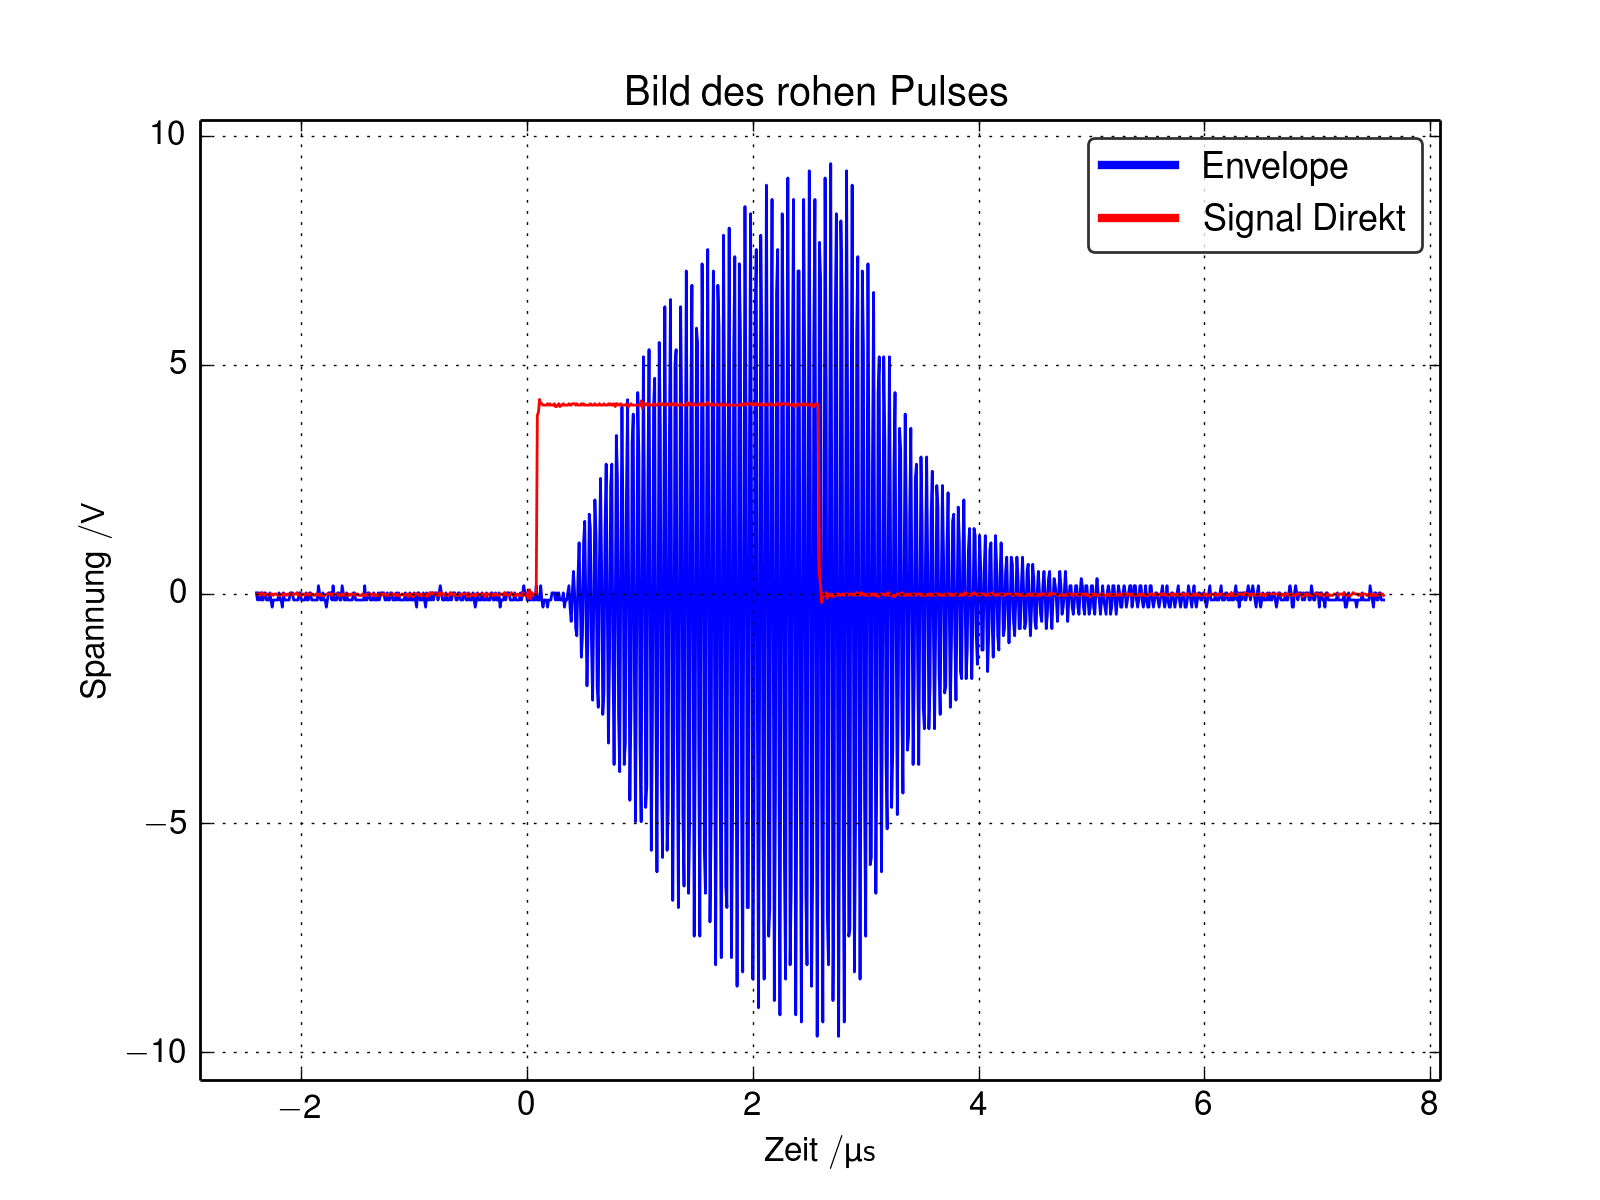
\includegraphics[width=\textwidth]{Figures/RohPuls1.png}
        \caption{Signal des elektromagnetischen Pulses.
          Sowohl direkt am Ausgang des Synthesizer als auch an der Probe
          gemessen.}
        \label{figRohPuls}
      \end{figure}


      
    \end{section}
    %%%%%%%%%%%%%%%%%%%%%%%%%%%%%
    
  \end{chapter}
  %%%%%%%%%%%%%%%%%%%%
  
  
  
  %%%%%%%%%%%%%%%%%%%%
  %%%%%%%%%%%%%%%%%%%%
  %%%%%%%%%%%%%%%%%%%%
  \begin{chapter}{Durchführung und Auswertung der Messdaten}
    \label{chp:Auswertung}
    Nachdem nun alles nach Anleitung aufgebaut und verkabelt ist und das Signal
    optimiert wurde, beginnen wir nun mit den eigentlichen Messungen dieses
    Versuches.
    
    %%%%%%%%%%%%%%%%%%%%%%%%%%%%%%
    %%%%%%%%%%%%%%%%%%%%%%%%%%%%%%
    %%%%%%%%%%%%%%%%%%%%%%%%%%%%%%
    \begin{section}{Offset der Spannungen}
      \label{chpOffset}
      Zunächst führen wir eine Messung ohne jegliches Signal durch um einen
      möglichen \textit{Offset} zu bestimmen.
      Dazu schalten wir die Messspannungen für \textit{Envelope}, \textit{Q} und
      \textit{I} am Oszilloskop ein, lassen aber das Signal am Synthesizer
      ausgeschaltet.
      \begin{figure}[hb]
        \centering
        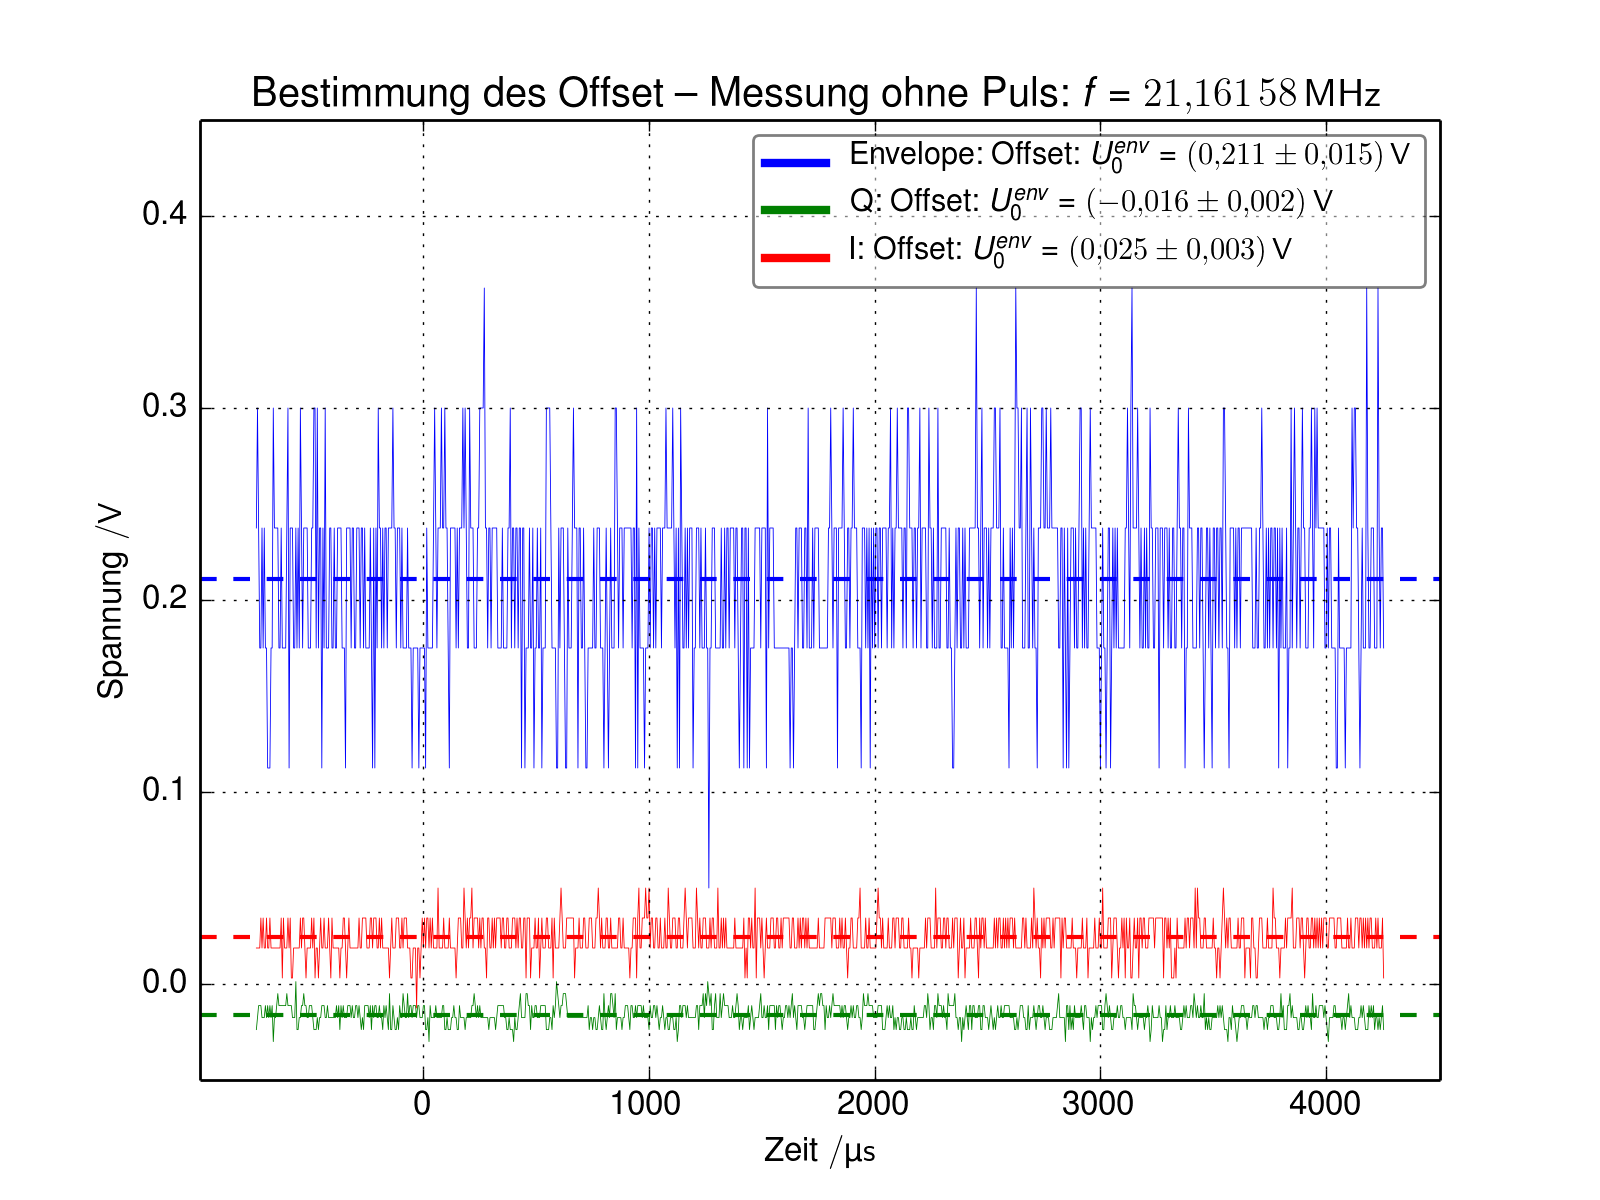
\includegraphics[width=1\textwidth]{Figures/Offset.png}
        \caption{Messdaten \textbf{ohne} eingeschalteten Puls zur
          \textit{Offset} - Messung.}
        \label{figOffset}
      \end{figure}

      Die von uns damit gemessenen Spannungen sind in \cref{figOffset} zusammen
      mit den berechneten Mittelwerten dargestellt.
      Alle hiernach genommenen Messwerte haben wir mit den gefundenen
      Offsets korrigiert.
      
    \end{section}
    %%%%%%%%%%%%%%%%%%%%%%%%%%%%%
    
    
    
    %%%%%%%%%%%%%%%%%%%%%%%%%%%%%%
    %%%%%%%%%%%%%%%%%%%%%%%%%%%%%%
    %%%%%%%%%%%%%%%%%%%%%%%%%%%%%%
    \begin{section}{Justierung der Pulszeiten}
      \label{chpPulszeiten}
      Um heraus zu finden welche Pulslängen einem $\pi$-, bzw.\
      $\frac{\pi}{2}$ - Puls entsprechen, messen wir Amplitude des
      Antwort - Signales während wir die Pulslänge variieren.
      Zunächst bestimmen wir den $\pi$ - Puls, indem wir eine Pulsdauer suchen,
      bei der das Antwort - Signal eine minimale Amplitude besitzt.
      Bei dieser Pulslänge löschen sich Puls und Antwort - Signal komplett aus.
      \todo{Warum?}
      Für unseren Aufbau haben wir hierbei eine Länge des $\pi$ - Pulses von
      $A_{len}=\SI{5.44}{\micro\second}$ gefunden.
      Für den $\frac{\pi}{2}$ - Puls gilt, dass dieser genau der halben Länge
      des $\pi$ - Pulses, also $A_{len}=\SI{2.72}{\micro\second}$, entspricht.
      
      \todo{Fertig?}
      \todo{oder ist das schon im aufbau gemacht worden?}
      
    \end{section}
    %%%%%%%%%%%%%%%%%%%%%%%%%%%%%
    
    
    
    %%%%%%%%%%%%%%%%%%%%%%%%%%%%%%
    %%%%%%%%%%%%%%%%%%%%%%%%%%%%%%
    %%%%%%%%%%%%%%%%%%%%%%%%%%%%%%
    \begin{section}[Free Induction Decay]{
        \underline{F}ree \underline{I}nduction \underline{D}ecay}
      \label{chpFID}
      Als nächstes optimieren wir das FID - Signal indem wir die Gradienten
      des Magnetfeldes so verstellen, dass das Profil möglichst einem
      exponentiellem Abfall entspricht.
      Da wir das Profil über das Oszilloskop nur nach Augenmaß einstellen
      konnten, entspricht das Profil leider nicht perfekt dem angestrebten
      exponentiellen Verlauf.
      Im Zeitraum von etwa $\SI{1.5}{\milli\second}$ bis
      $\SI{4.5}{\milli\second}$ konnten wir dennoch ein ausreichend
      gutes exponentielles Profil erreichen.
      An diesen zeitlichen Bereich passen wir \cref{eqFID}
      \begin{equation}
        \label{eqFID}
        M(\tau)=M_{0}\exp{\left(-\frac{\tau}{T_{2}^{*}}+c\right)},
      \end{equation}
      \todo{ist die Funktion okay oder soll ich das c wieder raus nehmen?}
      mit einer Versatzvariablen $c$ um den leicht verschobenen exponentiellen
      Abfall zu kompensieren, an.
      \Cref{figFIDenv} stellt das FID - Signal und die daran angepasste Kurve
      graphisch mit dem sowohl wir als auch unser Tutor einigermaßen zufrieden
      waren dar.
      \begin{figure}[htb]
        \centering
        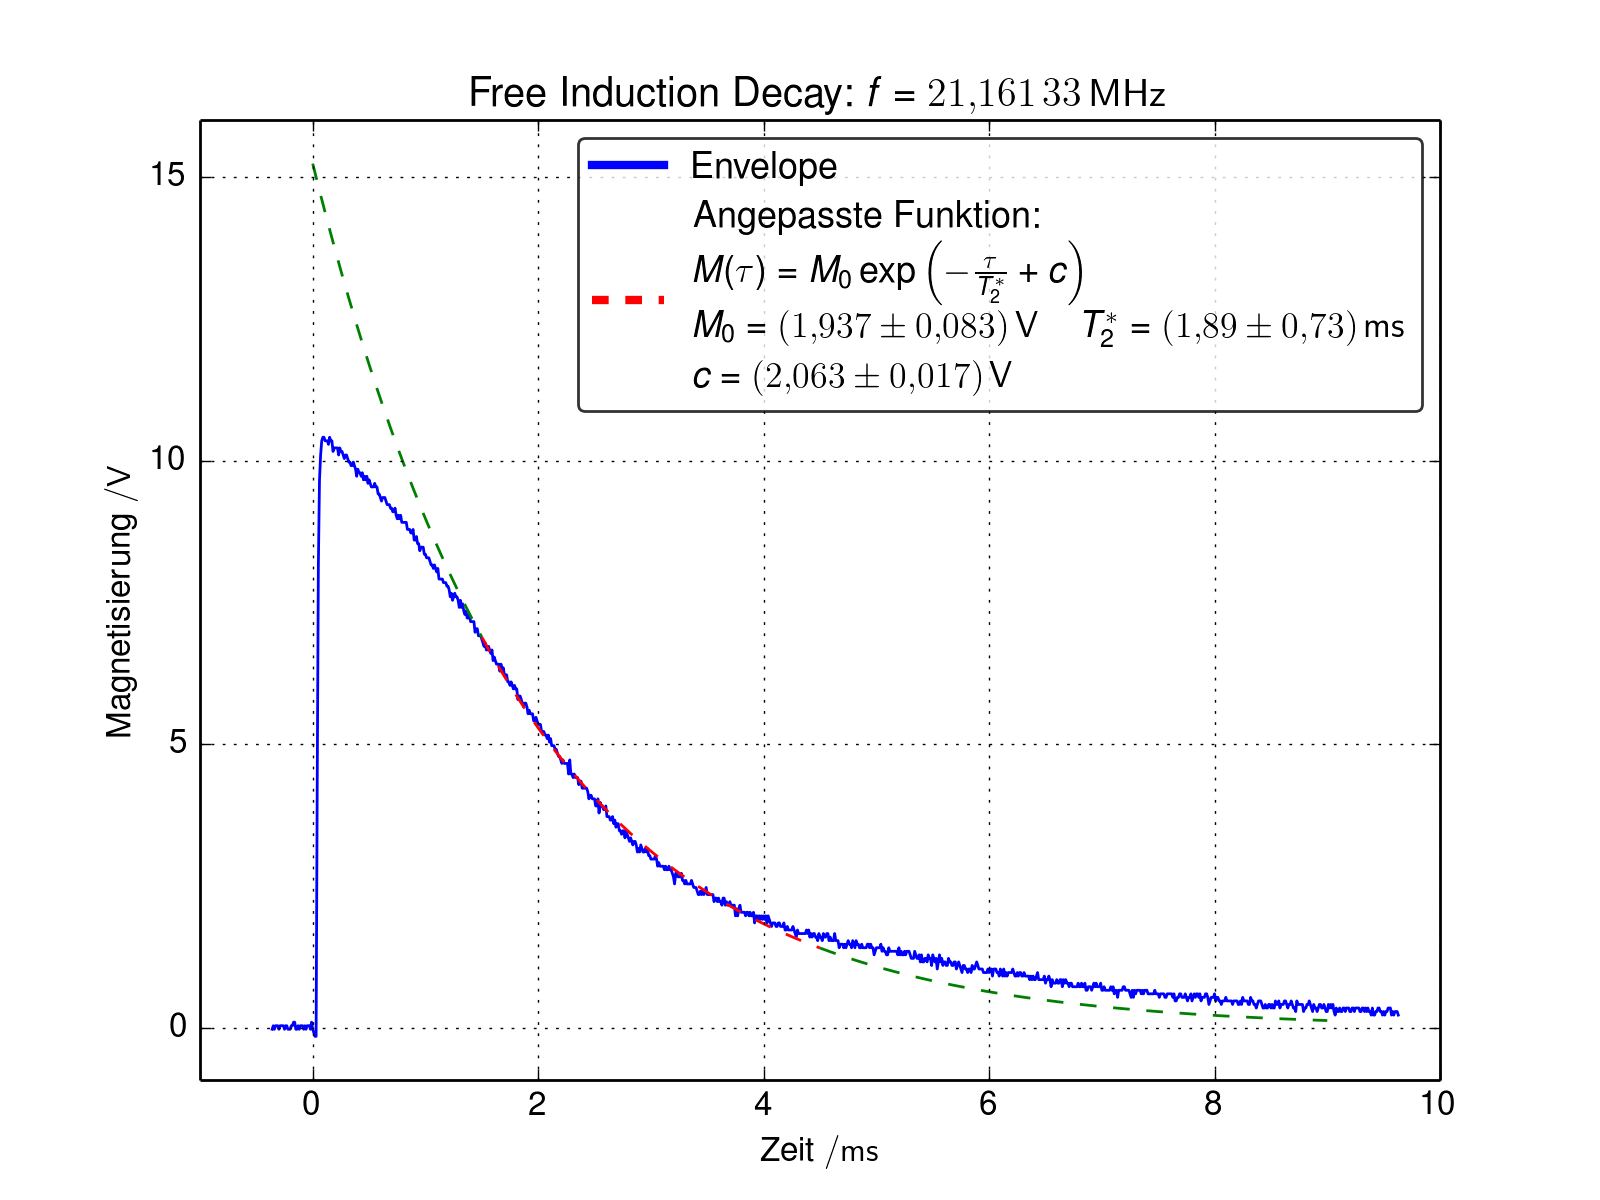
\includegraphics[width=.7\textwidth]{Figures/FID_env2.png}
        \caption{\textit{Free Induction Decay} Antwort - Signal und angepasste
          Zerfalls - Funktion.}
        \label{figFIDenv}
      \end{figure}
      
      Zu beginn des Versuches haben wir eine Resonanz der Lamorfrequenz von
      $\SI{21.16158}{\mega\hertz}$ gefunden.
      Da sich im laufe des Versuches etwas am FID - Profil verändert hat
      mussten wir nach einiger Zeit die Frequenz verändern um weiterhin die
      Resonanzfrequenz zu treffen.
      Daher haben wir dazu eine Frequenz von $\SI{21.16133}{\mega\hertz}$
      eingestellt.
      Bei welcher Frequenz eine Messung aufgenommen wurde ist jeweils im Titel
      der Graphiken festgehalten.
      \todo{fehlt noch was zu T2*. und ist das HIER tatsächlich richtig
        oder besser nachher wenn T2* tatsächlich gebraucht wird?}
      
%       \begin{figure}[htb]
%         \centering
%         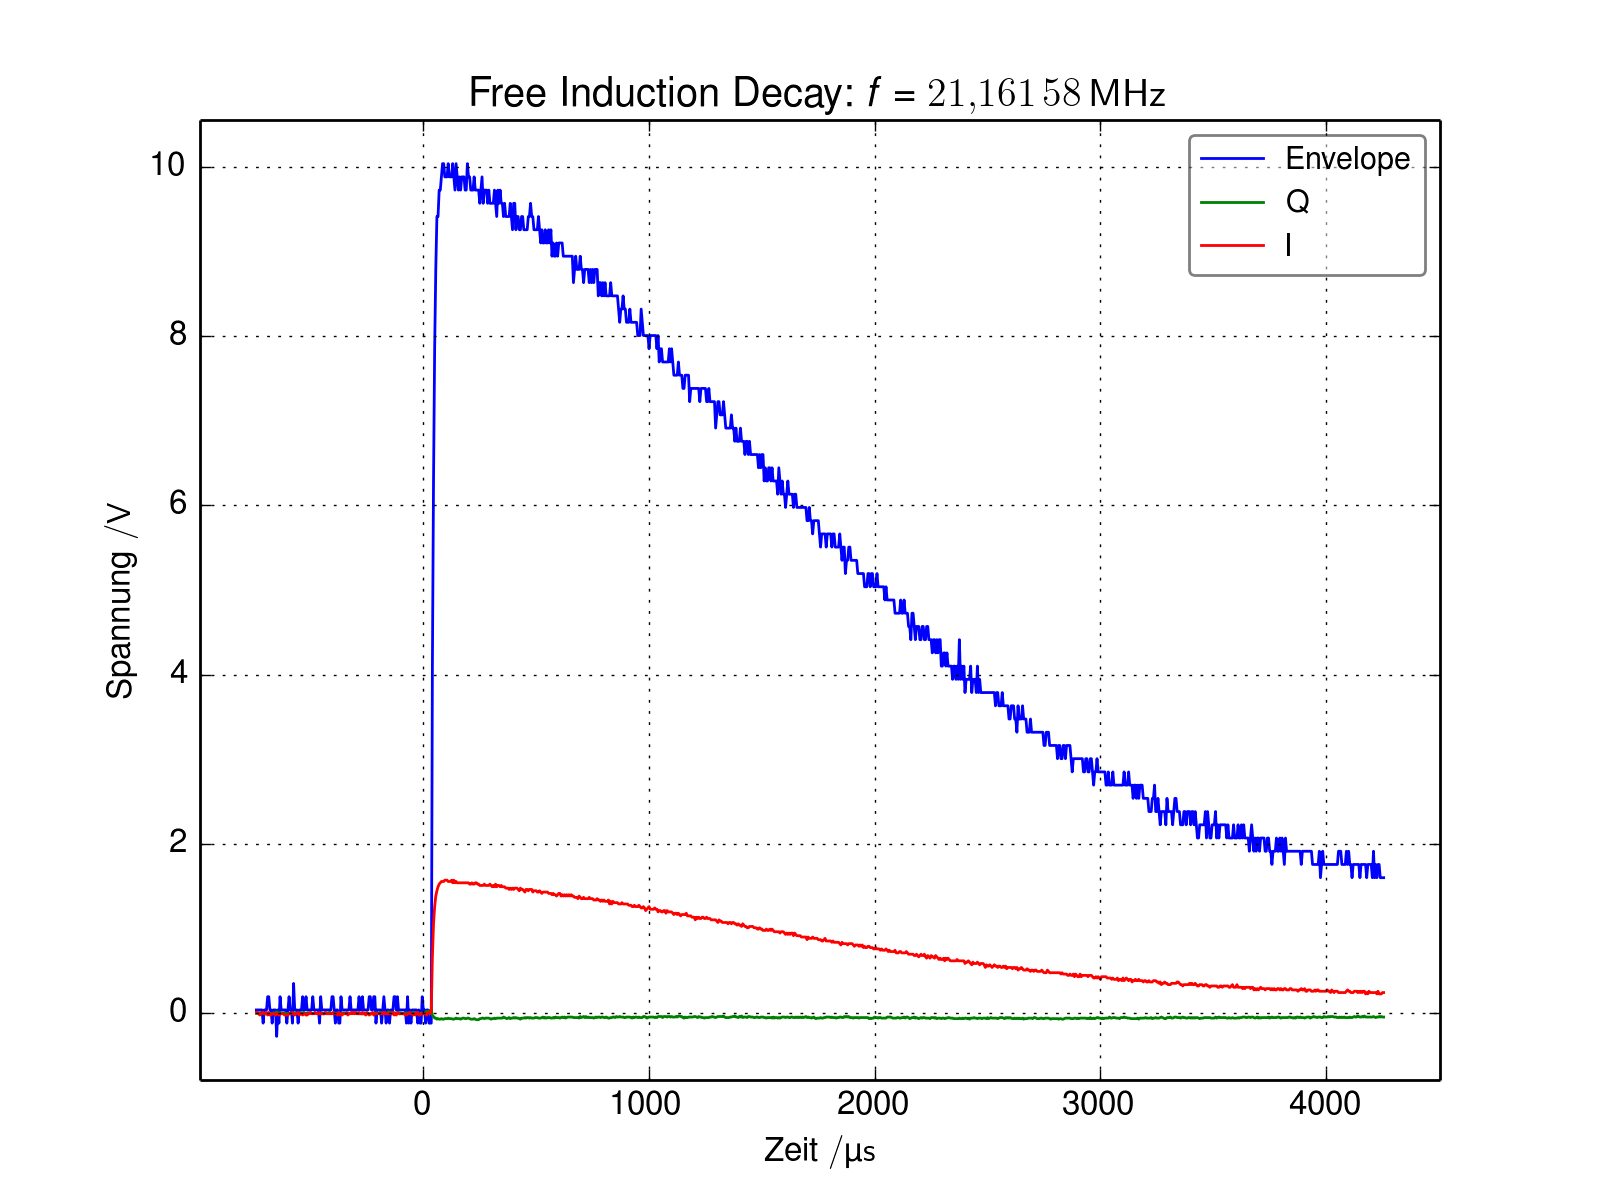
\includegraphics[width=\textwidth]{Figures/FID_env_Q_I0.png}
%         \caption{\textit{Free Induction Decay} Signal gemessen an der Probe.
%           Zusammen mit \textit{Q}-- und \textit{I}--Signal.}
%         \label{figFIDenvQI}
%       \end{figure}

      
      %%%%%%%%%%%%%%%%%%%%%%%%%%%%%%%%%%%%%%%
      %%%%%%%%%%%%%%%%%%%%%%%%%%%%%%%%%%%%%%%
      %%%%%%%%%%%%%%%%%%%%%%%%%%%%%%%%%%%%%%%
      \begin{subsection}[Effektive Transversale Relaxationszeit]
        {Effektive Transversale Relaxationszeit $T_{2}^{*}$}
        \label{chpEffTransRelax}
        Die effektive transversale Relaxationszeit $T_{2}^{*}$ setzt sich
        aus der inhomogenen transversalen Relaxationszeit
        $T_{2,\mathtt{inhom}}$ und der homogenen transversalen Relaxationszeit
        $T_{2}$ über \cref{eqEffektiveTransversaleRelaxationszeit} zusammen.
        \begin{equation}
          \label{eqEffektiveTransversaleRelaxationszeit}
          \frac{1}{T_{2}^{*}}=\frac{1}{T_{2,\mathtt{inhom}}}+\frac{1}{T_{2}}
        \end{equation}
        Aus dem FID - Signal lässt sich an dieser Stelle die effektive
        transversale Relaxationszeit $T_{2}^{*}$ direkt bestimmen.
        Dazu haben wir zuvor eine Funktion der Form von \cref{eqFID} an das
        Signal angepasst.
        Aus den somit gewonnenen Parametern der Anpassung erhalten wir nun
        die effektive transversale Relaxationszeit
        $T_{2}^{*}=\SI{1.89(73)}{\milli\second}$.
        
        In diesem Versuch wollen wir außerdem die inhomogene transversale
        Relaxationszeit $T_{2,\mathtt{inhom}}$ bestimmen indem wir zusätzlich
        zu der effektiven transversalen Relaxationszeit die homogene
        transversale Relaxationszeit $T_{2}$ über verschiedene
        Spinecho - Sequenzen bestimmen.
        Dazu aber später in \cref{chpHomoTransRelax} mehr.
        
      \end{subsection}
      %%%%%%%%%%%%%%%%%%%%%%%%%%%%%%%%%%%%%%%
      
    \end{section}
    %%%%%%%%%%%%%%%%%%%%%%%%%%%%%
    
    
    
    %%%%%%%%%%%%%%%%%%%%%%%%%%%%%%
    %%%%%%%%%%%%%%%%%%%%%%%%%%%%%%
    %%%%%%%%%%%%%%%%%%%%%%%%%%%%%%
    \begin{section}{Rabi--Oszillation}
      \label{chpRabi}
      Um die Rabi--Oszillation zu messen, benutzen wir einen Puls und variieren
      dessen Länge.
      Dabei messen wir die maximale Amplitude des Antwort - Signales und des
      In--Phase - Signales der Probe für jede eingestellte Pulslänge.
      Diese Messung wiederholen wir für eine leicht andere Frequenz.
      \todo{warum?}
      Um den Verlauf der Oszillation besser zu erkennen haben wir eine
      Betragsfunktion des Sinus angepasst und zusammen mit den Messdaten in
      \cref{figRabifreq12} abgebildet.
      \begin{figure}[htbp]
        \centering
        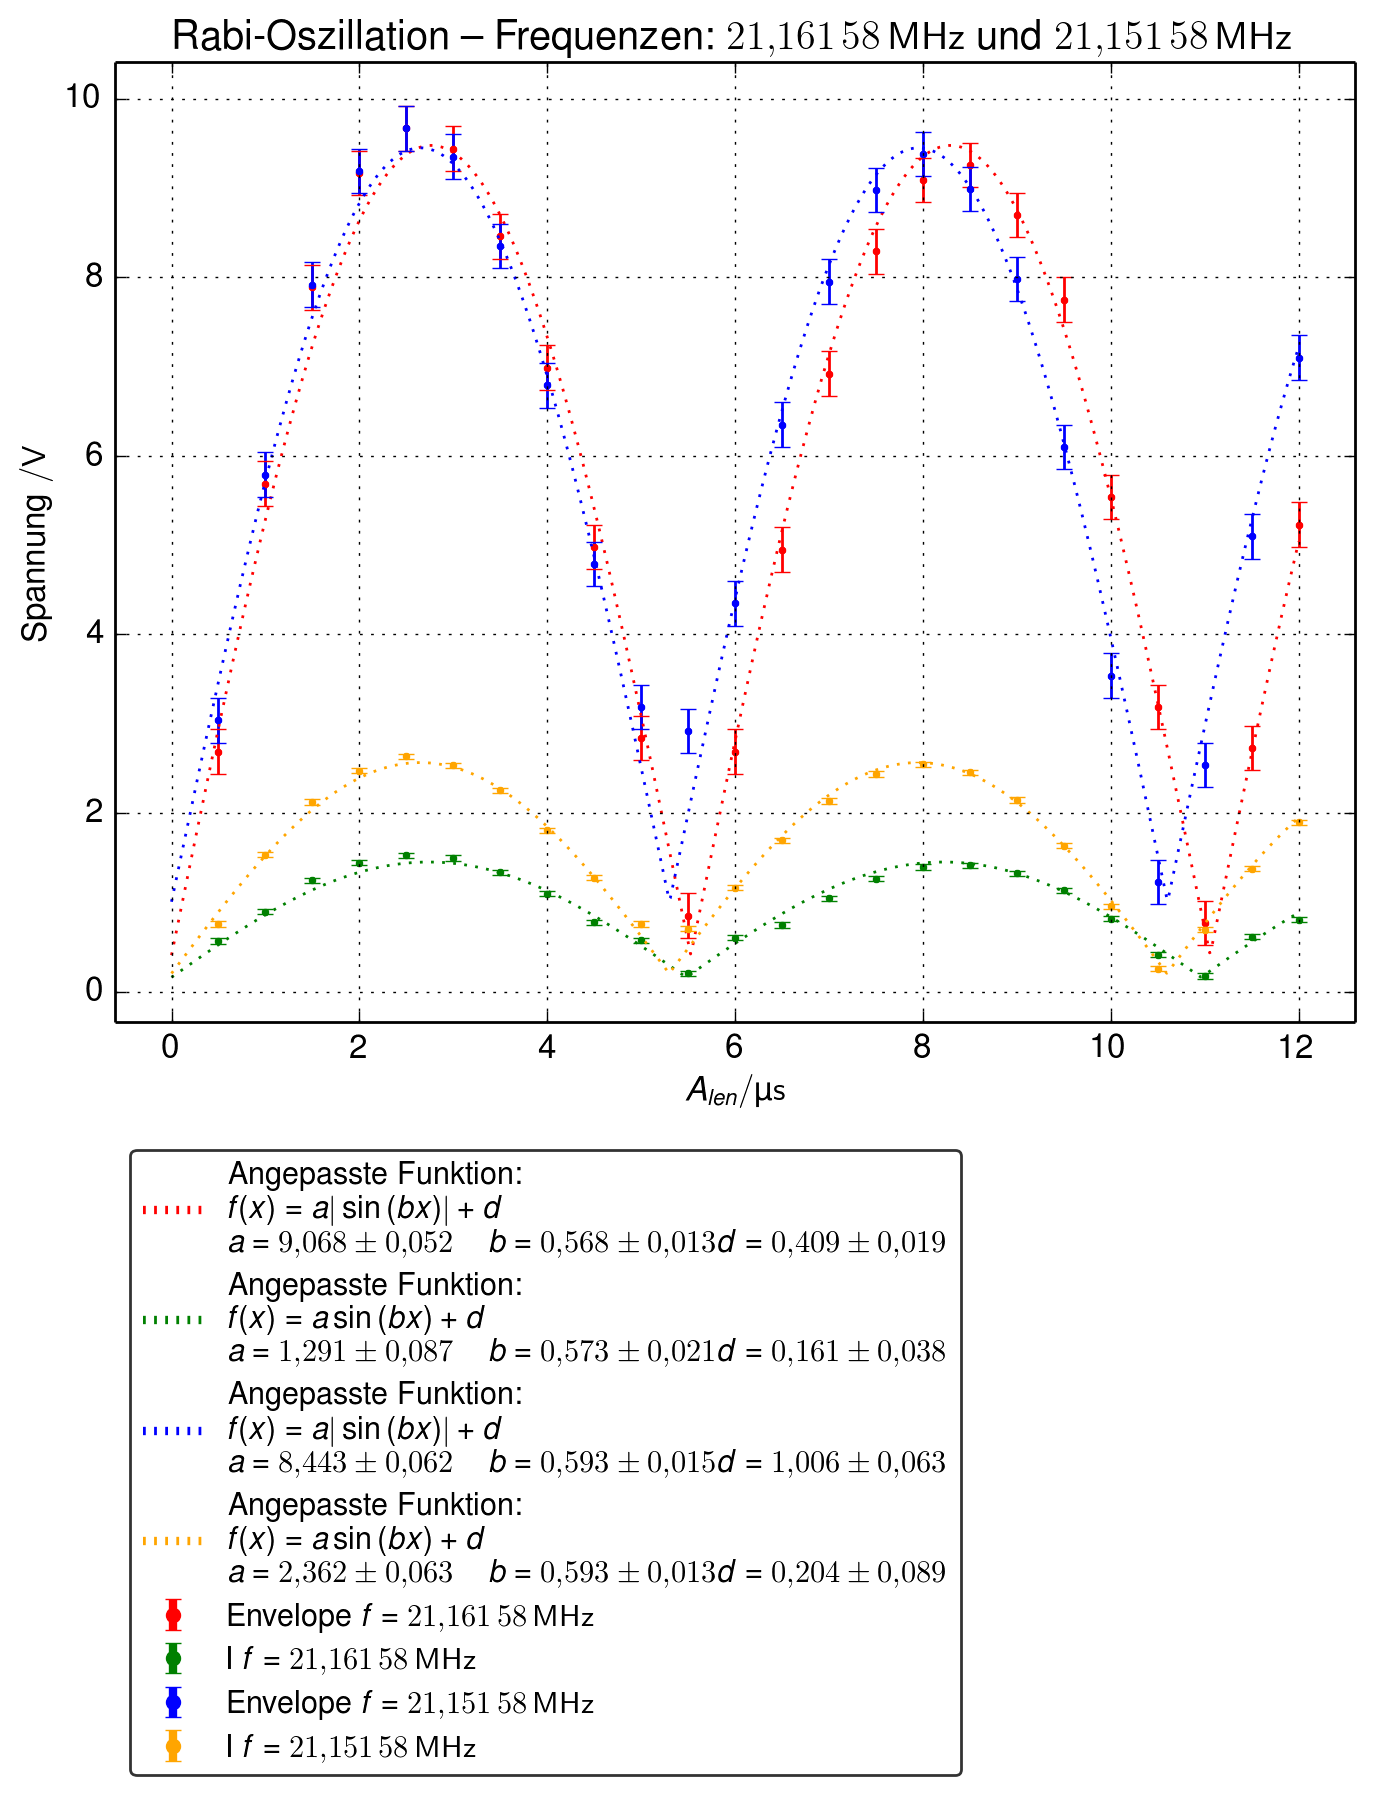
\includegraphics[width=\textwidth]{Figures/Rabi_freq12.png}
        \caption{Rabi--Oszillationen des Antwort - und In--Phase - Signales.}
        \label{figRabifreq12}
      \end{figure}
      
      Wie wir auch schon in der Theorie erwartet haben steigt die Amplitude
      des Antwort - Signales mit an sobald sich die Pulslänge dem
      $\frac{\pi}{2}$ - Puls nähert und dort ein Maximum annimmt.
      Für eine Pulslänge um die des $\pi$ - Pulses nimmt die Amplitude wieder
      ab um dann bei der Länge entsprechend eines $\frac{3\pi}{4}$ - Pulses
      wieder ein Maximum erreicht.
      Das In--Phase - Signal...
      \todo{haben wir bei den unteren Oszillationen ein vorzeichen übersehen
        oder soll das auch ein sinus betrag sein? Martin hat da eine normale
        sinus schwingung!}
      
    \end{section}
    %%%%%%%%%%%%%%%%%%%%%%%%%%%%%
    
    
    
    %%%%%%%%%%%%%%%%%%%%%%%%%%%%%%
    %%%%%%%%%%%%%%%%%%%%%%%%%%%%%%
    %%%%%%%%%%%%%%%%%%%%%%%%%%%%%%
    \begin{section}[Longitudinale Relaxationszeit]{
        Longitudinale Relaxationszeit $T_{1}$}
      \label{chpLongRelax}
      In diesem Versuchsteil wollen wir die longitudinale Relaxationszeit
      $T_{1}$ messen.
      Dazu stehen uns stehen uns in diesem Versuch zwei verschiedene Methoden
      zur Verfügung die wir hier beiden durchführen und anschließend
      vergleichen wollen.
      Die Relaxationszeit $T_{1}$ kann hierbei sowohl mit der
      Sättigungs--Zurückgewinnungs- als auch mit der Polarisations--
      Zurückgewinnungs - Methode über die Höhe des FID - Signales bestimmt werden.
      
      
      %%%%%%%%%%%%%%%%%%%%%%%%%%%%%%%%%%%%%%%
      %%%%%%%%%%%%%%%%%%%%%%%%%%%%%%%%%%%%%%%
      %%%%%%%%%%%%%%%%%%%%%%%%%%%%%%%%%%%%%%%
      \begin{subsection}{Sättigungs--Zurückgewinnung}
        \label{chpLongRelaxSaettigung}
        Bei der Sättigungs--Zurückgewinnungs - Methode wird zunächst mit einem
        $\frac{\pi}{2}$ - Puls... \todo{was genau passiert hier? Erklärungen!}
        
        Die für diese Methode benutzte Sequenz ist in \cref{eqSaettigungSequenz}
        noch einmal notiert.
        \begin{equation}
          \label{eqSaettigungSequenz}
          \frac{\pi}{2} \rightarrow \mathtt{FID} \rightarrow
          \tau \frac{\pi}{2} \rightarrow \mathtt{FID}
        \end{equation}
        Wir variieren für diese Messung die Verzögerungszeit $\tau$ in einem
        Bereich von $\SI{10}{\milli\second}$ bis $\SI{750}{\milli\second}$
        und messen jeweils die maximale Amplitude des Antwort - Signales nach
        den zweiten Puls.
        Die aufgenommenen Messwerte der maximalen Spannung sind in
        \cref{figSaettigung} gegen die variierte Verzögerungszeit $\tau$
        aufgetragen.
        \begin{figure}[htb]
          \centering
          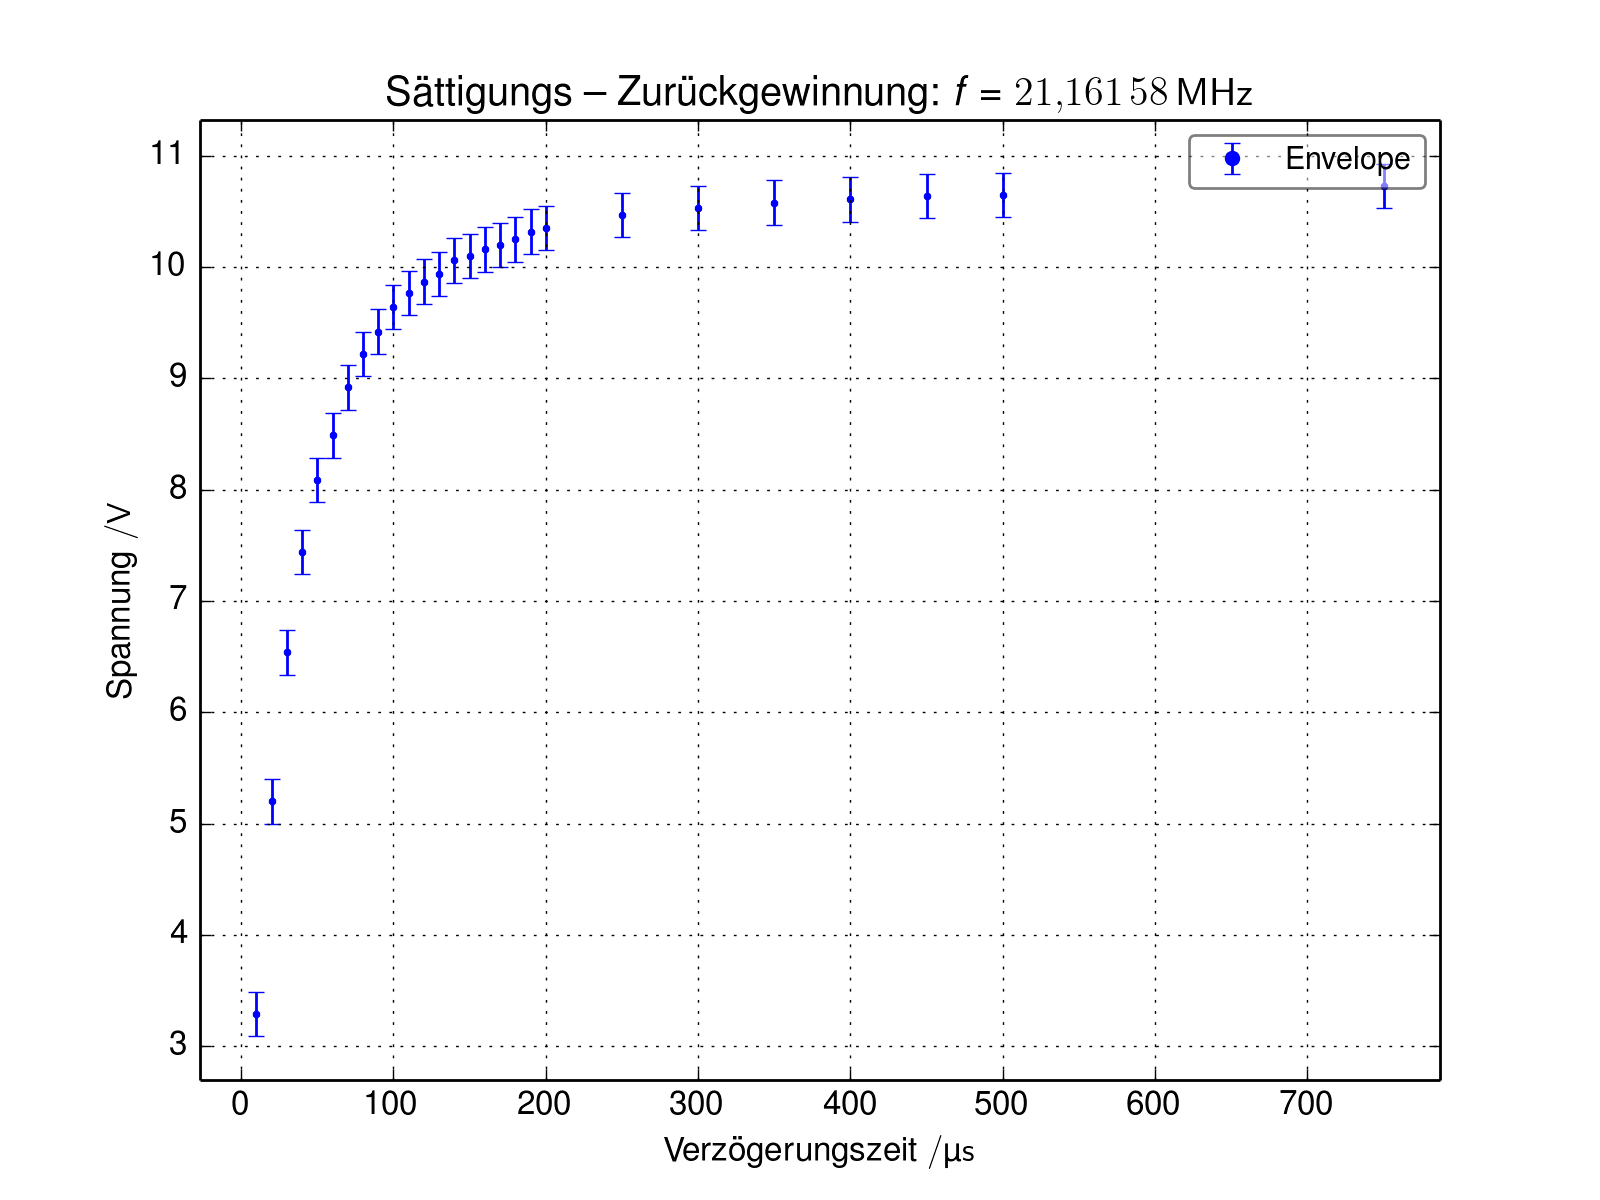
\includegraphics[width=\textwidth]
          {Figures/SaettigungsZurueckgewinnung.png}
          \caption{Verlauf der maximalen Spannung des Antwort - Signales bei der
            Sättigungs--Zurückgewinnungs - Methode.}
          \label{figSaettigung}
        \end{figure}
        
        Um nun die longitudinale Relaxationszeit $T_{1}$ zu bestimmen,
        passen wir eine Funktion der Form von \cref{eqSaettigung} an die
        genommenen Messwerte an.
        \begin{equation}
          \label{eqSaettigung}
          M(\tau)=M_{0}\left(1-\exp\left(-\frac{\tau}{T_{1}}\right)\right)
        \end{equation} \todo{Woher kommt diese Form?}
        Die angepasste Funktion ist in \cref{figSaettigung} zusammen mit den
        Daten abgebildet.
        Aus den Parametern dieser Anpassung erhalten wir nun die zu bestimmende
        longitudinale Relaxationszeit $T_{1}=\SI{32.096(54)}{\milli\second}$
        und eine maximale Spannung $M_{0}=\SI{10.338(39)}{\volt}$.
        Es ist aber deutlich zu erkennen, dass eine Funktion der Form von
        \cref{eqSaettigung} den Verlauf nicht optimal approximiert, da die
        Funktion bereits nach einigen Messpunkten nicht mehr dem tatsächlichen
        Verlauf der Daten entspricht.
        \todo{Ideen warum oder wie es besser wäre?}
        
      \end{subsection}
      %%%%%%%%%%%%%%%%%%%%%%%%%%%%%%%%%%%%%%%
      
      
      
      %%%%%%%%%%%%%%%%%%%%%%%%%%%%%%%%%%%%%%%
      %%%%%%%%%%%%%%%%%%%%%%%%%%%%%%%%%%%%%%%
      %%%%%%%%%%%%%%%%%%%%%%%%%%%%%%%%%%%%%%%
      \begin{subsection}{Polarisations--Zurückgewinnung}
        \label{chpLongRelaxPolarisation}
        \todo{Erklärungen!}
        Die Messungen bei dieser Methode ähneln denen der Sättigungs--
        Zurückgewinnungs - Methode bis auf die verwendete Sequenz und die an die
        Messwerte angepasste Funktion.
        
        Für die Polarisations--Zurückgewinnung - Methode verwenden wir
        \cref{eqPolarisationSequenz} als Sequenz von Pulsen, bei der wieder die
        Verzögerungszeit $\tau$ im gleichen Bereich variiert wird.
        \begin{equation}
          \label{eqPolarisationSequenz}
          \pi \rightarrow \tau \frac{\pi}{2} \rightarrow \mathtt{FID}
        \end{equation} \todo{Warum? woher?}
        An die gemessenen Spannungen passen wir bei der Polarisations--
        Zurückgewinnungs - Methode eine Funktion von der Form der
        \cref{eqPolarisation} an.
        \begin{equation}
          \label{eqPolarisation}
          M(\tau)=M_{0}\left(1-2\cdot\exp\left(-\frac{\tau}{T_{1}}\right)\right)
        \end{equation} \todo{Warum? woher?}
        Sowohl die Messwerte als auch die angepasste Funktion sind, wie zuvor,
        in \cref{figPolarisation} dargestellt und gegen die variierte
        Verzögerungszeit $\tau$ aufgetragen.
        \begin{figure}[htb]
          \centering
          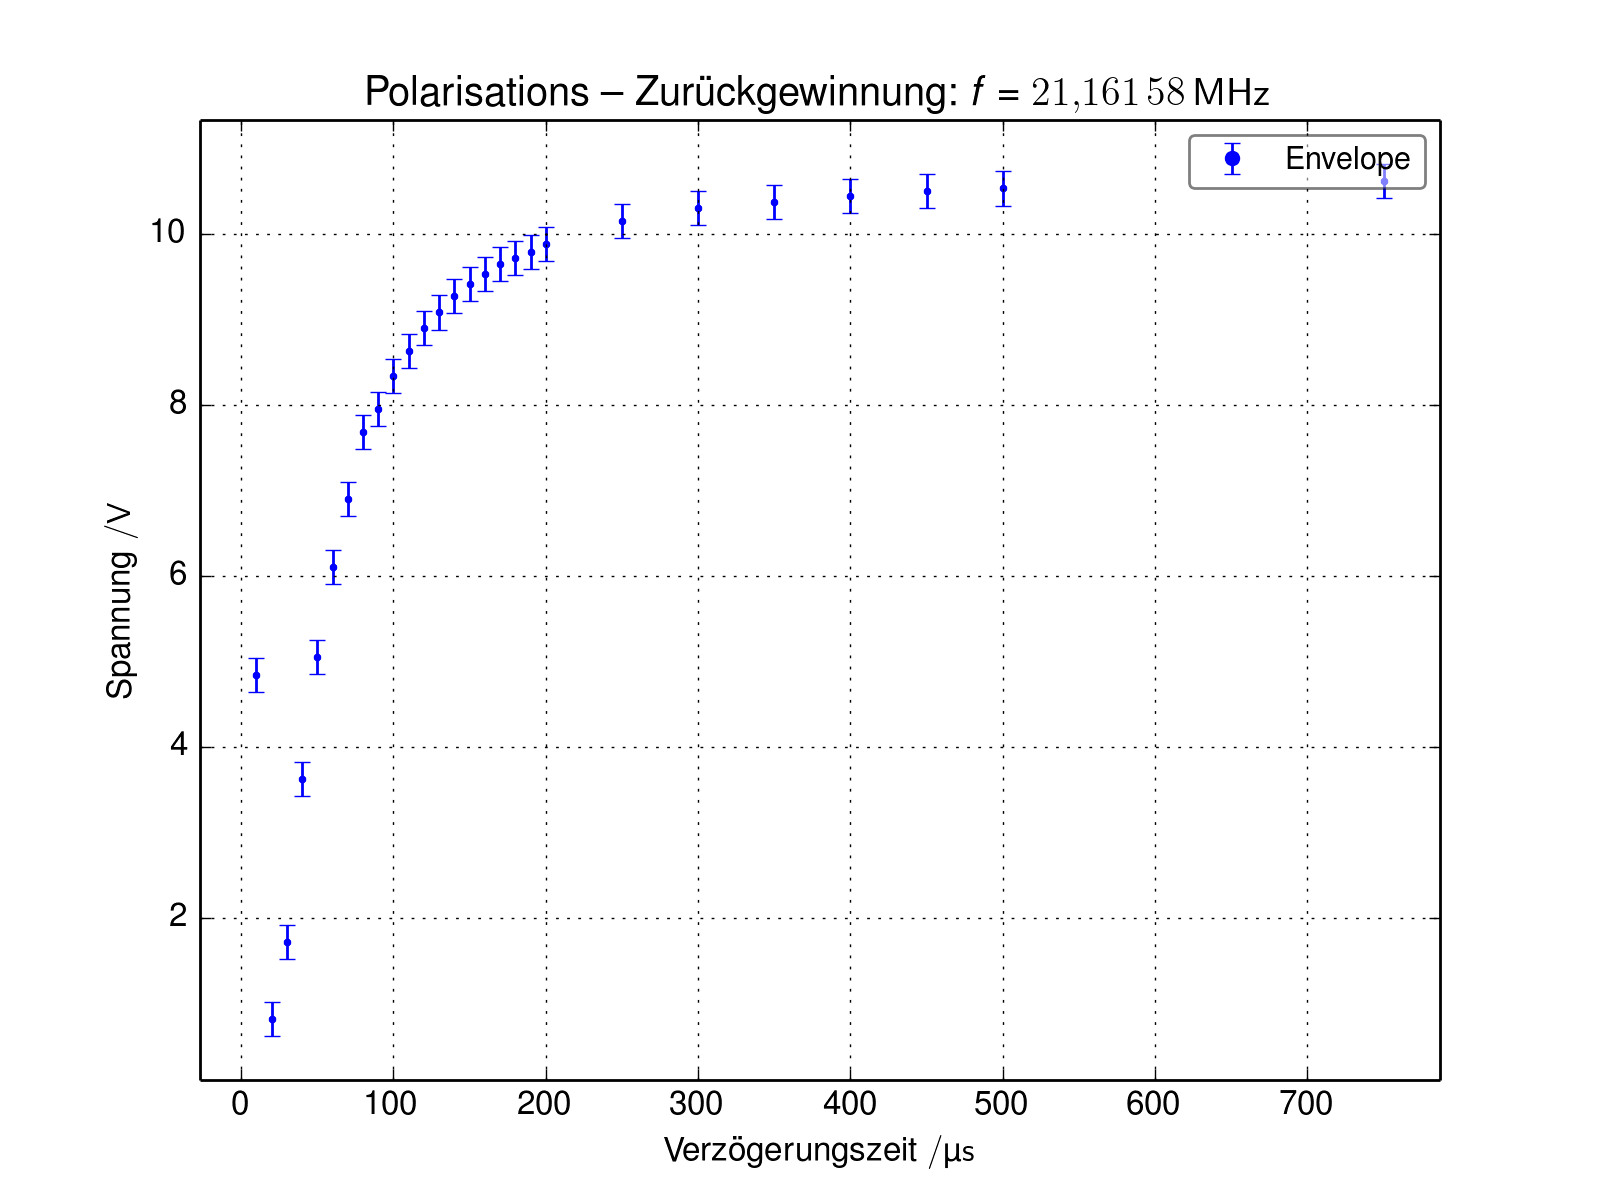
\includegraphics[width=\textwidth]
          {Figures/PolarisationsZurueckgewinnung.png}
          \caption{Verlauf der maximalen Spannung des Antwort - Signales bei der
            Polarisations--Zurückgewinnungs - Methode.}
          \label{figPolarisation}
        \end{figure}
        
        Aus den Parametern der Anpassung von \cref{eqPolarisation} erhalten
        wir nun die longitudinale Relaxationszeit
        $T_{1}=\SI{34,474(27)}{\milli\second}$ und $M_{0}=\SI{9,885(3)}{\volt}$.
        \todo{und? gefällt uns die Funktion?}
        
      \end{subsection}
      %%%%%%%%%%%%%%%%%%%%%%%%%%%%%%%%%%%%%%%
      
      \todo[inline]{Vergleiche beide Methoden! aber was genau soll man da sagen
      bzw.\ vergleichen?}
      
    \end{section}
    %%%%%%%%%%%%%%%%%%%%%%%%%%%%%
    
    
    
    %%%%%%%%%%%%%%%%%%%%%%%%%%%%%%
    %%%%%%%%%%%%%%%%%%%%%%%%%%%%%%
    %%%%%%%%%%%%%%%%%%%%%%%%%%%%%%
    \begin{section}[Homogene Transversale Relaxationszeit]{
        Homogene Transversale Relaxationszeit $T_{2}$}
      \label{chpHomoTransRelax}
      Wie zuvor in \cref{chpFID} erwähnt, möchten wir in diesem Versuch neben
      der dort bestimmten effektiven transversalen Relaxationszeit $T_{2}^{*}$
      auch die homogene transversale Relaxationszeit $T_{2}$ bestimmen.
      
      Dazu benutzen wir sog.\ \textit{Spinecho} - Sequenzen.
      Für diesen Versuch stehen uns dabei drei verschiedene Spinecho - Sequenzen
      zur Verfügung die im folgenden durchgeführt werden.
      
      %%%%%%%%%%%%%%%%%%%%%%%%%%%%%%%%%%%%%%%
      %%%%%%%%%%%%%%%%%%%%%%%%%%%%%%%%%%%%%%%
      %%%%%%%%%%%%%%%%%%%%%%%%%%%%%%%%%%%%%%%
      \begin{subsection}{Hahn--Spinecho - Sequenz}
        \label{chpHomoTransRelaxHahn}
        Zunächst befassen wir uns mit der \textit{Hahn--Spinecho} - Sequenz
        (\cref{eqHahnSequenz}).
        \begin{equation}
          \label{eqHahnSequenz}
          \frac{\pi}{2} \rightarrow \tau \pi
        \end{equation}
        Hierbei senden wir erst einen $\frac{\pi}{2}$ - Puls und nach einer
        Verzögerungszeit $\tau$ einen $\pi$ - Puls.
        
        \Cref{figHahnBsp1,figHahnBsp2} zeigen für zwei unterschiedliche
        Verzögerungszeiten beispielhaft wie das Antwort - Signal dieser
        Spinecho - Sequenz auf dem Oszilloskop aussieht.
        
        Um die homogene transversale Relaxationszeit $T_{2}$ nun zu bestimmen
        messen wir die maximale Amplitude des Echo - Signales bei verschiedenen
        Verzögerungszeiten $\tau$.
        An die damit erhaltenen Messwerte passen wir nun eine exponentielle
        Zerfalls - Funktion der Form von \cref{eqHomo} an.
        \begin{equation}
          \label{eqHomo}
          M(\tau)=M_{0}\exp\left(-\frac{\tau}{T_{2}}\right)
        \end{equation}
        Aus den Parametern dieser Anpassung erhalten wir somit die homogene
        transversale Relaxationszeit $T_{2}=\SI{9.833(65)}{\milli\second}$.
        Messdaten und angepasste Funktion zusammen mit den gefundenen
        Parametern sind in \cref{figHahn} gegen die variierte Verzögerungszeit
        $\tau$ aufgetragen.
        \begin{figure}[htb]
          \centering
          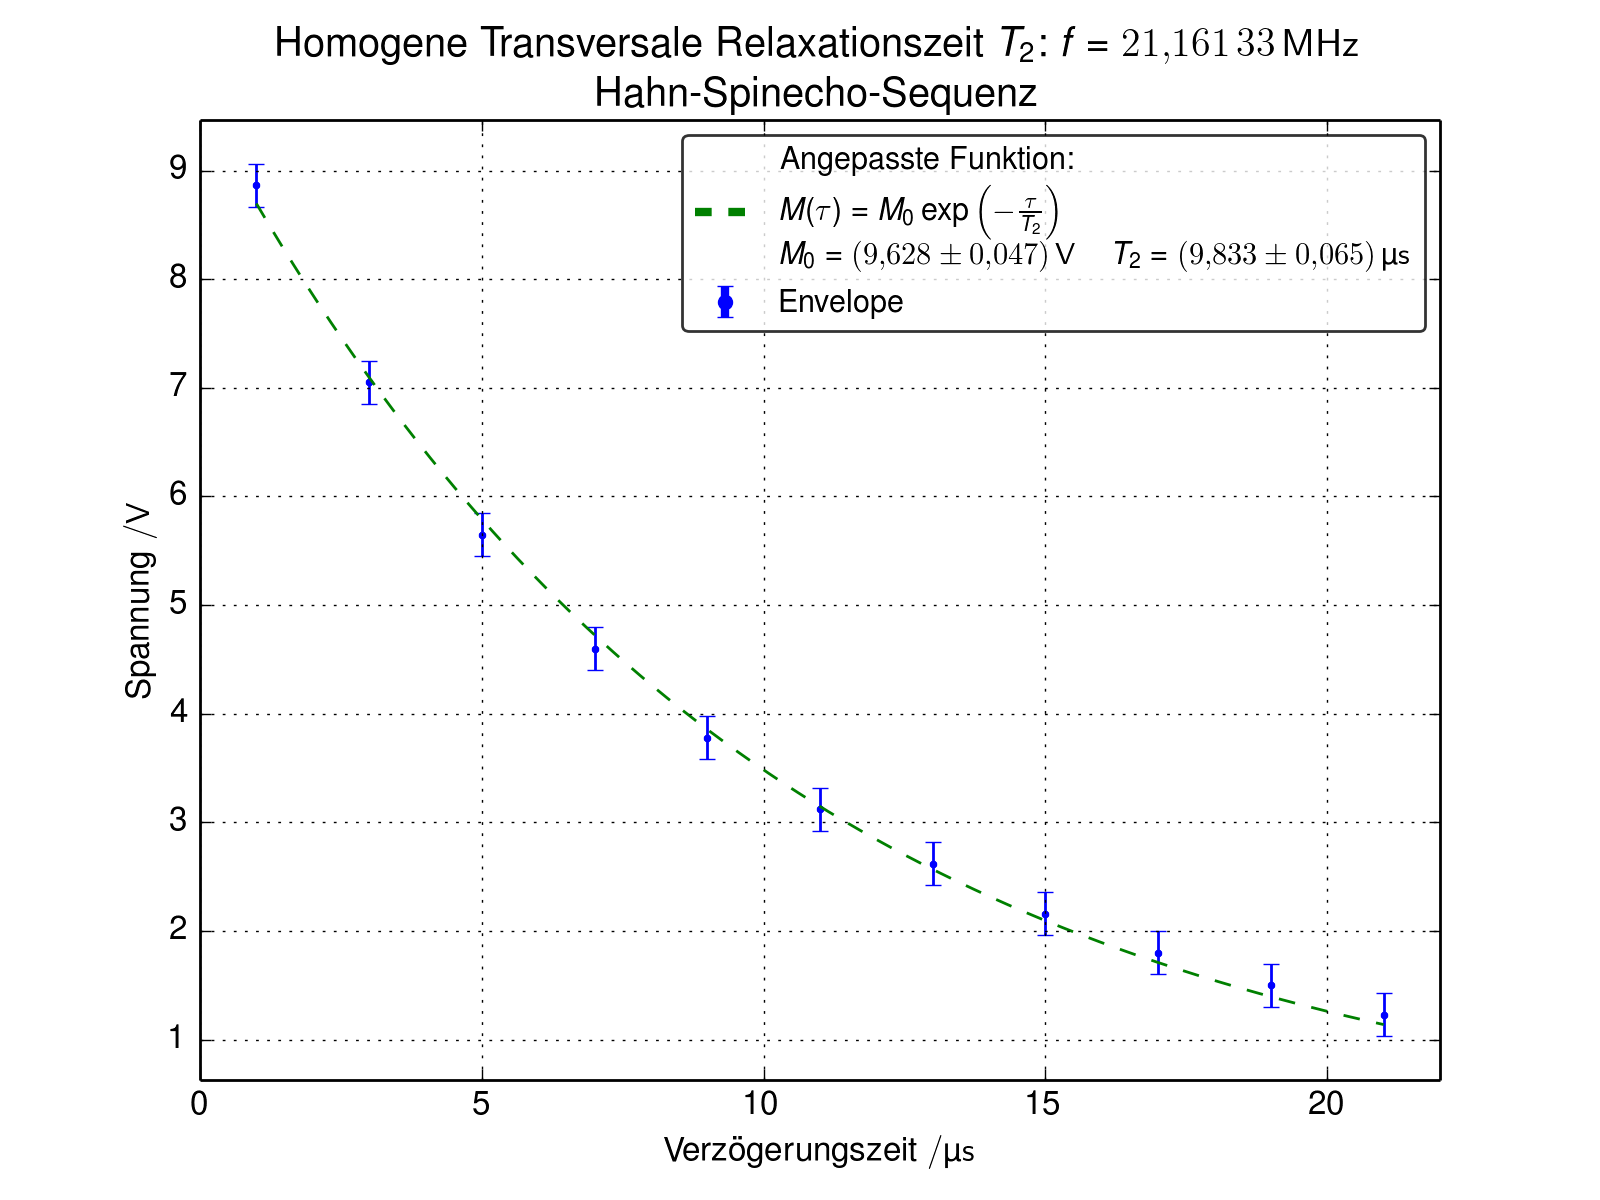
\includegraphics[width=\textwidth]
          {Figures/HomoTransRelax_Hahn.png}
          \caption{Verlauf der maximalen Spannung des Echo - Signales bei der
            Hahn--Spinecho - Sequenz.}
          \label{figHahn}
        \end{figure}
        \begin{figure}[htb]
          \centering
          \begin{minipage}{.48\textwidth}
            \centering
            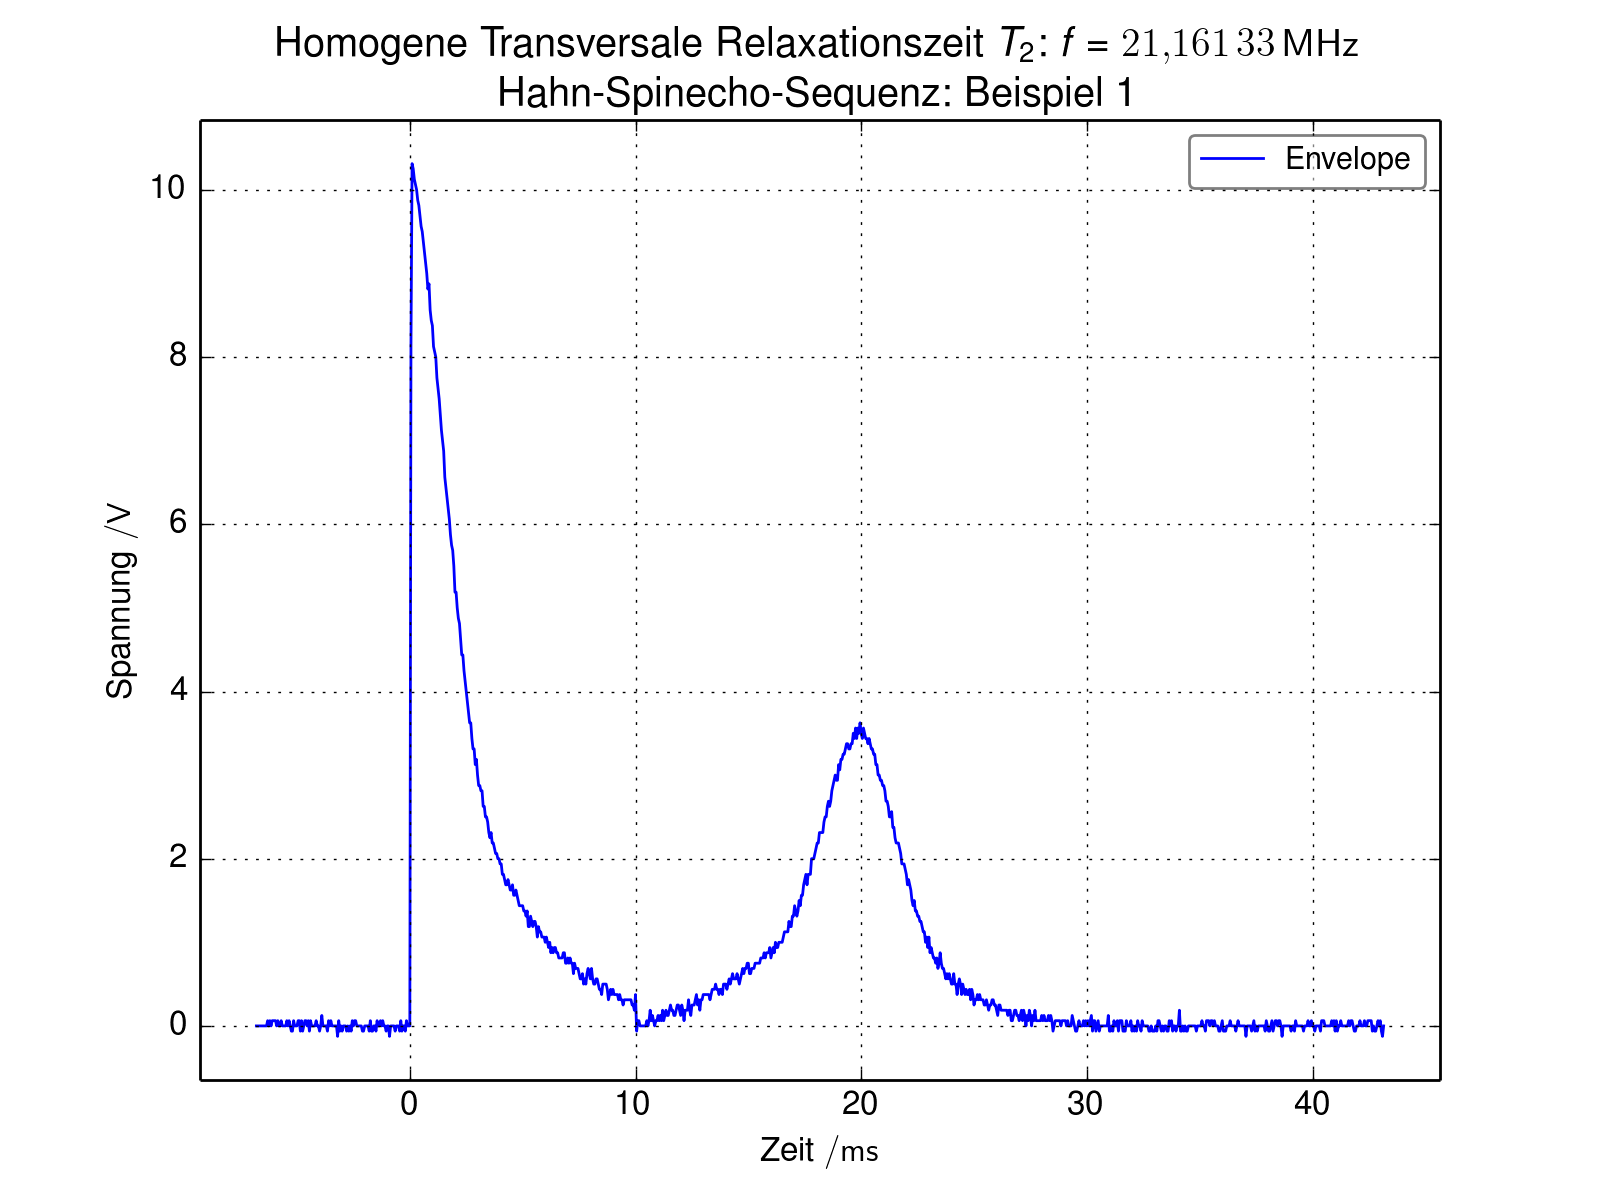
\includegraphics[width=\textwidth]
            {Figures/HomoTransRelax_Hahn_beispiel0.png}
            \caption{Beispiel eines Antwort - Signales bei der
              Hahn--Spinecho - Sequenz.}
            \label{figHahnBsp1}
          \end{minipage}\quad
          \begin{minipage}{.48\textwidth}
            \centering
            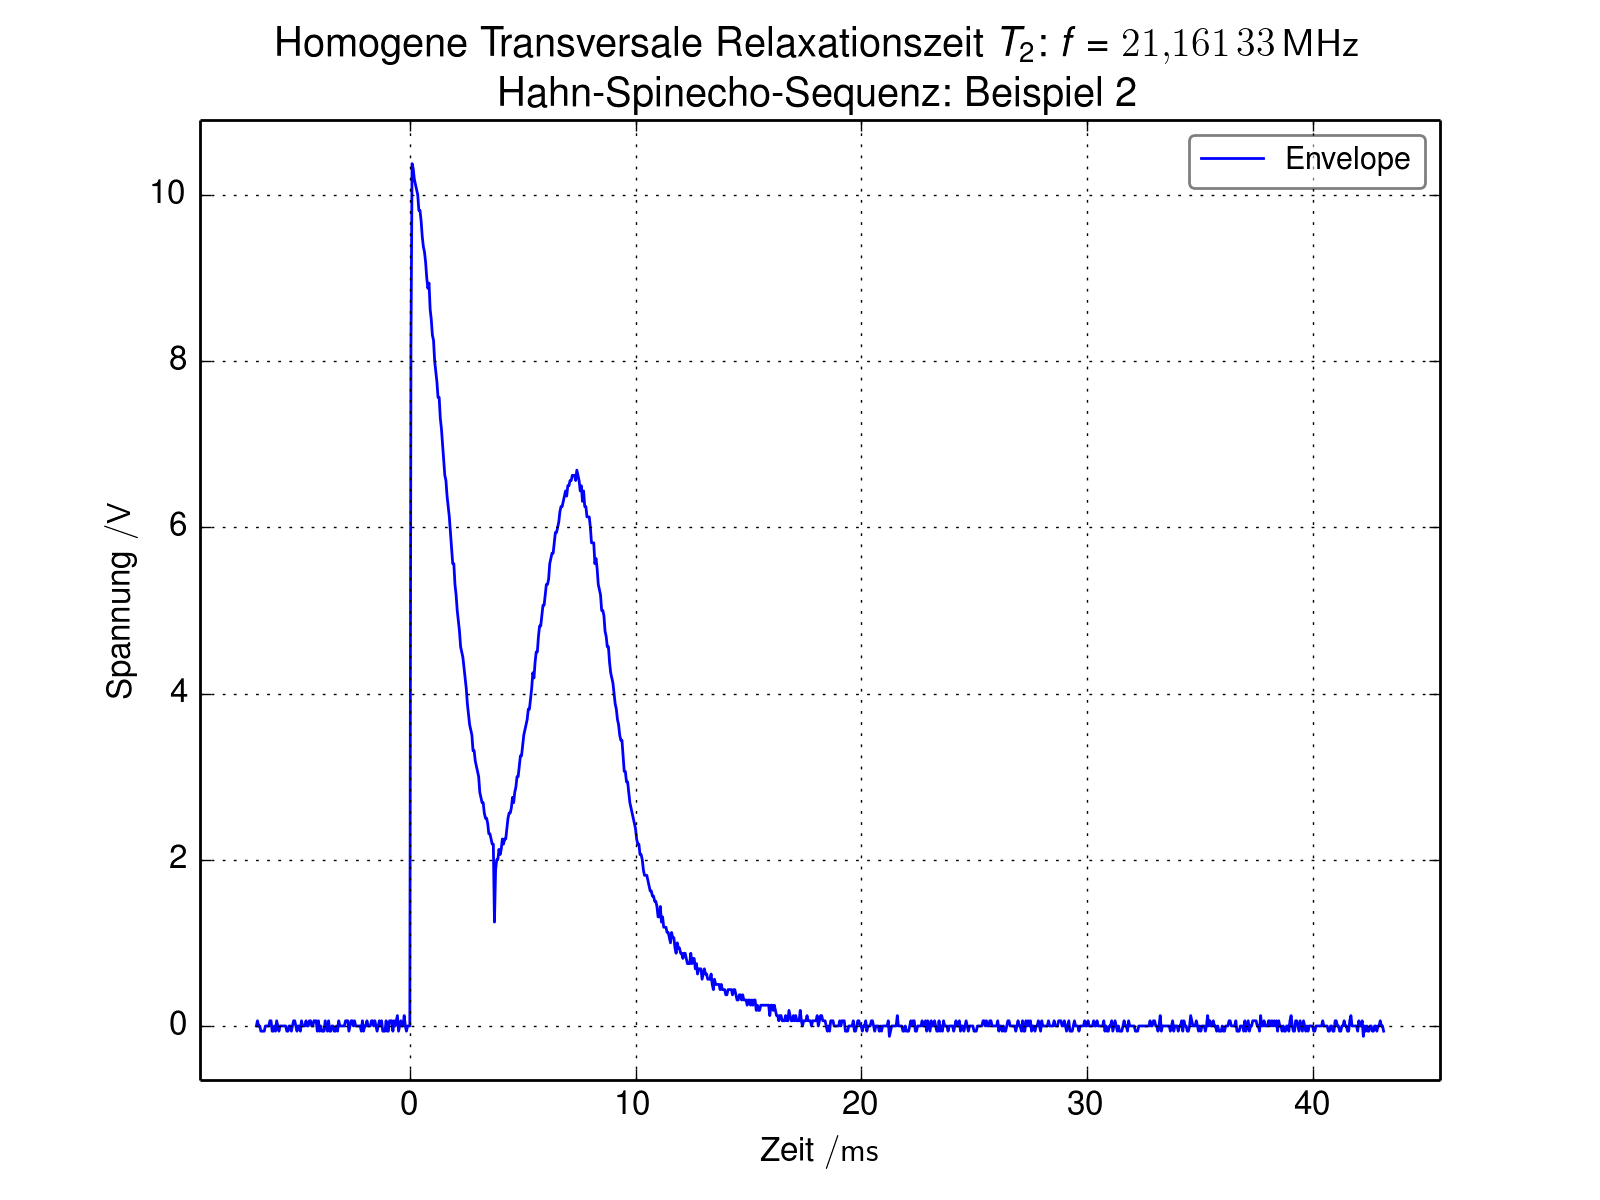
\includegraphics[width=\textwidth]
            {Figures/HomoTransRelax_Hahn_beispiel1.png}
            \caption{Beispiel eines Antwort - Signales bei der
              Hahn--Spinecho - Sequenz.}
            \label{figHahnBsp2}
          \end{minipage}
        \end{figure}
        
      \end{subsection}
      %%%%%%%%%%%%%%%%%%%%%%%%%%%%%%%%%%%%%%%
      
      
      
      %%%%%%%%%%%%%%%%%%%%%%%%%%%%%%%%%%%%%%%
      %%%%%%%%%%%%%%%%%%%%%%%%%%%%%%%%%%%%%%%
      %%%%%%%%%%%%%%%%%%%%%%%%%%%%%%%%%%%%%%%
      \begin{subsection}{Carr--Purcell--Spinecho - Sequenz}
        \label{chpHomoTransRelaxCarr}
        Bei der Messung der homogenen transversalen Relaxationszeit mithilfe der
        \textit{Carr--Purcell} - Sequenz benutzen wir eine Sequenz von
        Pulsen mit einem immer wiederkehrenden Muster.
        Die Carr--Purcell - Sequenz ist in \cref{eqCarrSequenz} anschaulich
        dargestellt.
        \begin{equation}
          \label{eqCarrSequenz}
          \frac{\pi}{2} \rightarrow \tau\pi \rightarrow 2\tau\pi \rightarrow
          2\tau\pi \rightarrow 2\tau\pi \rightarrow \ldots
        \end{equation}
        Das Antwort - Signal sieht, auf dem Oszilloskop betrachtet, wie in
        \cref{figCarrBsp} dargestellt aus.
        
        Um nun mit dieser Sequenz die homogene transversale Relaxationszeit
        zu bestimmen müssen wir zunächst einmal die lokalen Maxima der Messung
        bestimmen.
        Dazu verwenden wir \texttt{Python}, genauer gesagt die
        \texttt{signal.find\_peaks\_cwt} Funktion des \texttt{Python.scipy}
        Modules.
        An dieser Stelle sollten wir erwähnen, dass, auch nach einigem
        Feintuning der \texttt{signal.find\_peaks\_cwt} Funktion, es uns leider
        nicht bei allen lokalen Maxima perfekt gelungen ist ihre Position zu
        finden.
        Dennoch sollte das erreichte Ergebnis ausreichen um die notwendigen
        Rechnungen durchzuführen.
        
        Die homogene transversale Relaxationszeit $T_{2}$ kann nun bestimmt
        werden, indem eine exponentielle Zerfalls - Funktion der Form
        von \cref{eqHomo} an die lokalen Maxima angepasst wird.
        Das erste Maximum wird für alle Messungen nicht bei der Anpassung der
        Funktion beachtet, da es sich bei diesem Extrempunkt nicht um ein
        Echo sondern um das Signal der eigentlichen Anregung handelt.
        Aus den Parametern der angepassten Funktion erhalten wir
        $T_{2}=\SI{13.986(4)}{\milli\second}$.
        \begin{figure}[htb]
          \centering
          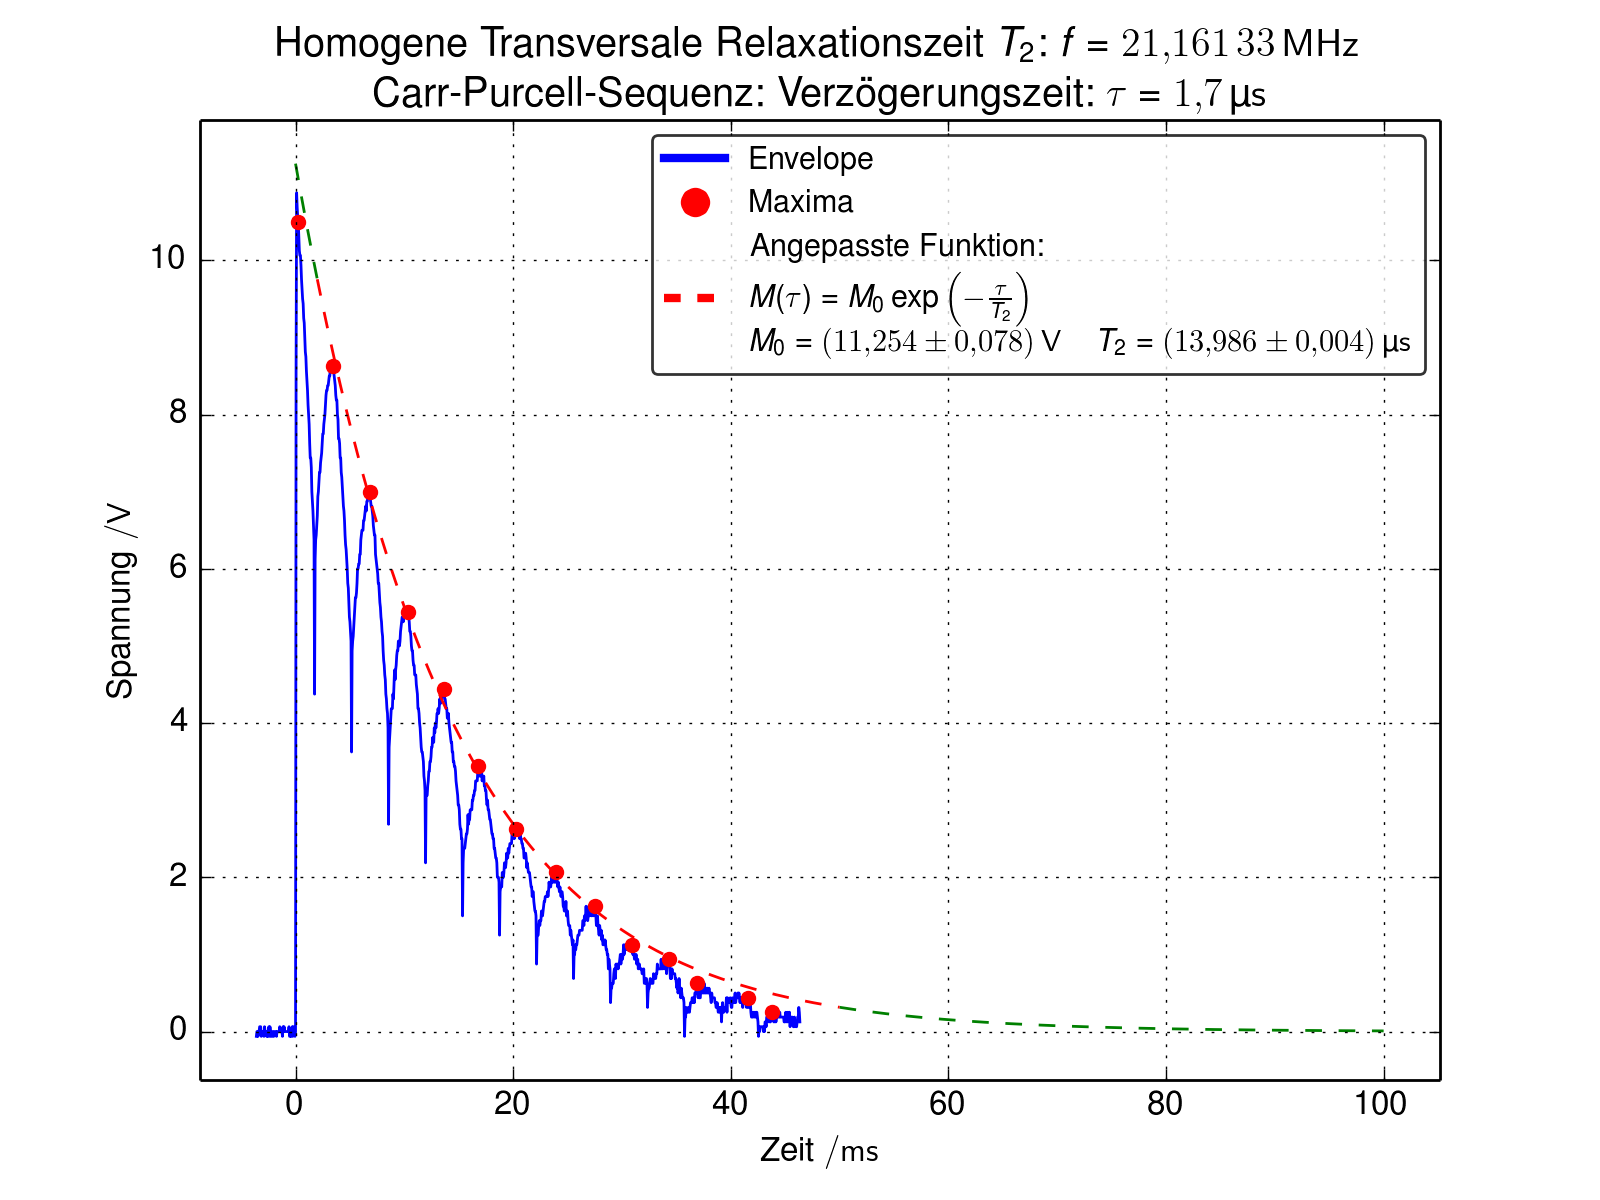
\includegraphics[width=\textwidth]
          {Figures/HomoTransRelax_Carr0.png}
          \caption{Verlauf der lokalen Maxima des Antwort - Signales für die
            Carr--Purcell - Sequenz bei einer Verzögerungszeit von
            $\tau = \SI{1.7}{\micro\second}$.}
          \label{figCarrBsp}
        \end{figure}
        
        Zusätzlich haben wir in bei diesem Versuchsteil das Antwort - Signal
        dieser Sequenz bei verschiedenen Verzögerungszeiten $\tau$ und
        einem veränderten Magnetfeld - Gradienten beobachtet.
        Beim variieren der Verzögerungszeit konnten wir feststellen, dass sich
        $T_{2}$ ebenfalls entsprechend ändert.
        Auch beim ändern des Magnetfeld - Gradienten hat sich $T_{2}$
        verändert.
        Allerdings waren die Änderungen hier deutlich schwächer als bei
        unterschiedlichen Verzögerungszeiten.
        Die kleinste Änderung von $T_{2}$ haben wir bei den beiden Messungen mit
        unterschiedlichen Magnetfeld - Gradienten gefunden.
        Wie sich $T_{2}$ mit der Verzögerungszeit und dem
        Magnetfeld - Gradienten ändert ist in \cref{tabCarr} notiert.
        \todo[inline]{Erklärungen??? Idee warum das so ist??}
        \begin{table}[htb]
          \centering
          \rowcolors{2}{}{lightgray!30}
          \begin{tabular}{c|c|c}
            Magnetfeld - Gradient & $\tau$ & $T_{2}$ \\ \hline
            Normal & \SI{1.7}{\micro\second} & \SI{13.986(4)}{\milli\second} \\
            Normal & \SI{2.0}{\micro\second} & \SI{15.206(36)}{\milli\second} \\
            Normal & \SI{2.6}{\micro\second} & \SI{17.172(19)}{\milli\second} \\
            $Z^{-1}$ & \SI{2.6}{\micro\second} & \SI{18.567(48)}{\milli\second} \\
            $X^{-1}$ & \SI{2.6}{\micro\second} & \SI{18.326(53)}{\milli\second} \\
          \end{tabular}
          \caption{Verhalten von $T_{2}$ bei verschiedenen Verzögerungszeiten
            $\tau$ und umgepoltem Z-bzw.\ X-Gradient des Magnetfeldes
            ($Z^{-1}$ und $X^{-1}$).}
          \label{tabCarr}
        \end{table}
        
      \end{subsection}
      %%%%%%%%%%%%%%%%%%%%%%%%%%%%%%%%%%%%%%%
      
      
      \newpage
      %%%%%%%%%%%%%%%%%%%%%%%%%%%%%%%%%%%%%%%
      %%%%%%%%%%%%%%%%%%%%%%%%%%%%%%%%%%%%%%%
      %%%%%%%%%%%%%%%%%%%%%%%%%%%%%%%%%%%%%%%
      \begin{subsection}{Meiboom--Gill--Spinecho - Sequenz}
        \label{chpHomoTransRelaxMG}
        Die dritte und letzte Sequenz, mit der die homogene transversale
        Relaxationszeit $T_{2}$ in diesem Versuch gemessen werden soll, ist die
        \textit{Meiboom--Gill} - Sequenz (\cref{eqMGSequenz}).
        \begin{equation}
          \label{eqMGSequenz}
          \frac{\pi}{2} \rightarrow \tau \pi_{+} \rightarrow 2\tau \pi_{-}
          \rightarrow 2\tau \pi_{+} \rightarrow 2\tau \pi_{-} \rightarrow
          2\tau \pi_{+} \rightarrow \ldots
        \end{equation}
        Mit dieser Sequenz ist schnell zu erkennen, dass sich die Echos deutlich
        länger halten.
        Einen Vergleich der Echo - Signale der Carr--Purcell - und der
        Meiboom--Gill - Sequenz haben wir in den \cref{figMG_env0,figMG_env1}
        grafisch dargestellt.
        Genau wie bei der Carr--Purcell - und der Hahn--Spinecho - Sequenz
        passen wir auch hier wieder eine Funktion der Form von \cref{eqHomo}
        an die lokalen Maxima an.
        Allerdings können wir, ähnlich wie bei der Justierung des
        FID - Signales in \cref{chpFID}, auch hier erkennen, dass der Verlauf der
        Maxima nicht optimal einem exponentiellen Zerfall folgt.
        Die mit den Parametern erhaltenen homogenen transversalen
        Relaxationszeiten für verschiedene Verzögerungszeiten $\tau$ haben wir
        in \cref{tabMG} notiert.
        \begin{table}[htb]
          \centering
          \rowcolors{2}{}{lightgray!30}
          \begin{tabular}{c|c|c}
            $\tau$ & $T_{2}$ (Meiboom--Gill) & $T_{2}$ (Carr--Purcell) \\ \hline
            \SI{1.6}{\micro\second} &
            \SI{25.159(84)}{\milli\second} & \SI{13.587(5)}{\milli\second} \\
            \SI{3.0}{\micro\second} &
            \SI{28.423(73)}{\milli\second} & \SI{18.767(62)}{\milli\second} \\
          \end{tabular}
          \caption{Verhalten von $T_{2}$ bei verschiedenen Verzögerungszeiten
            $\tau$ für die Meiboom--Gill - und Carr--Purcell - Sequenz.}
          \label{tabMG}
        \end{table}
        \begin{figure}[htb]
          \centering
          \begin{minipage}{.48\textwidth}
            \centering
            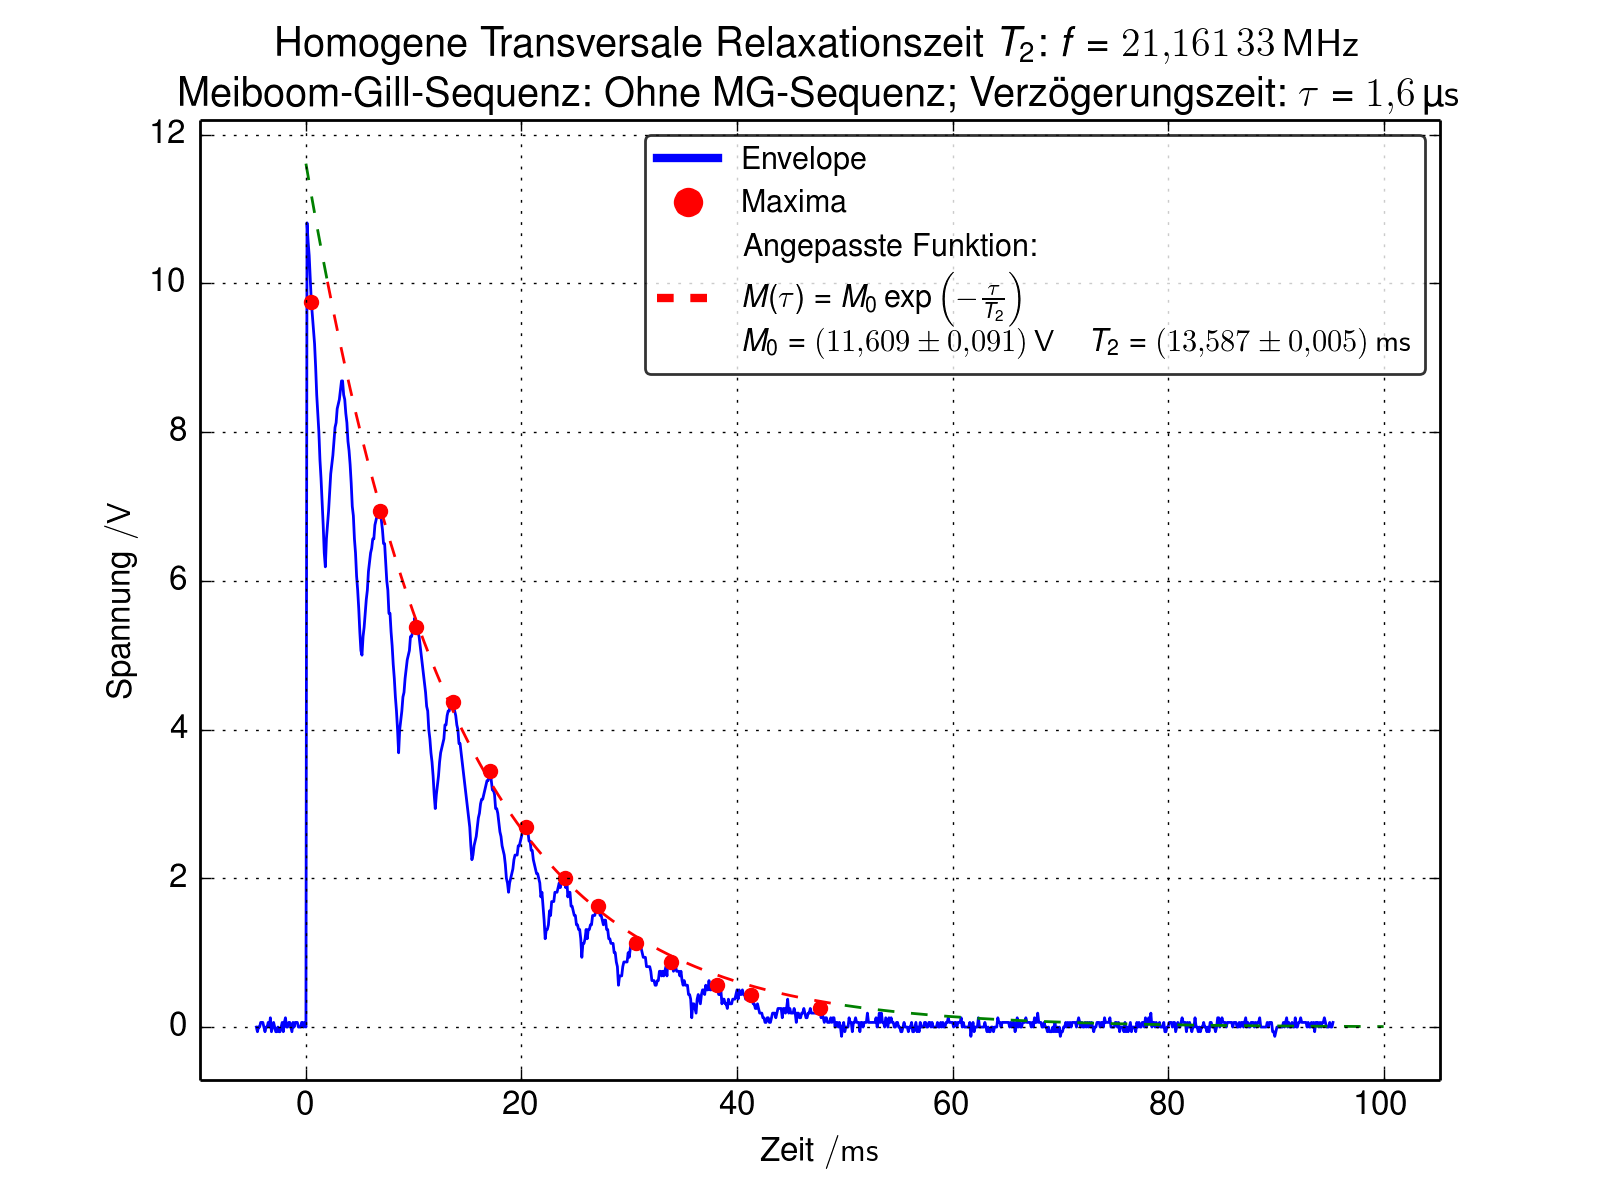
\includegraphics[width=\textwidth]
            {Figures/HomoTransRelax_MG_env0.png}
            \caption{Verlauf der lokalen Maxima des Antwort - Signales für die
              Carr--Purcell - Sequenz bei $\tau = \SI{1.6}{\micro\second}$.}
            \label{figMG_env0}
          \end{minipage}\quad
          \begin{minipage}{.48\textwidth}
            \centering
            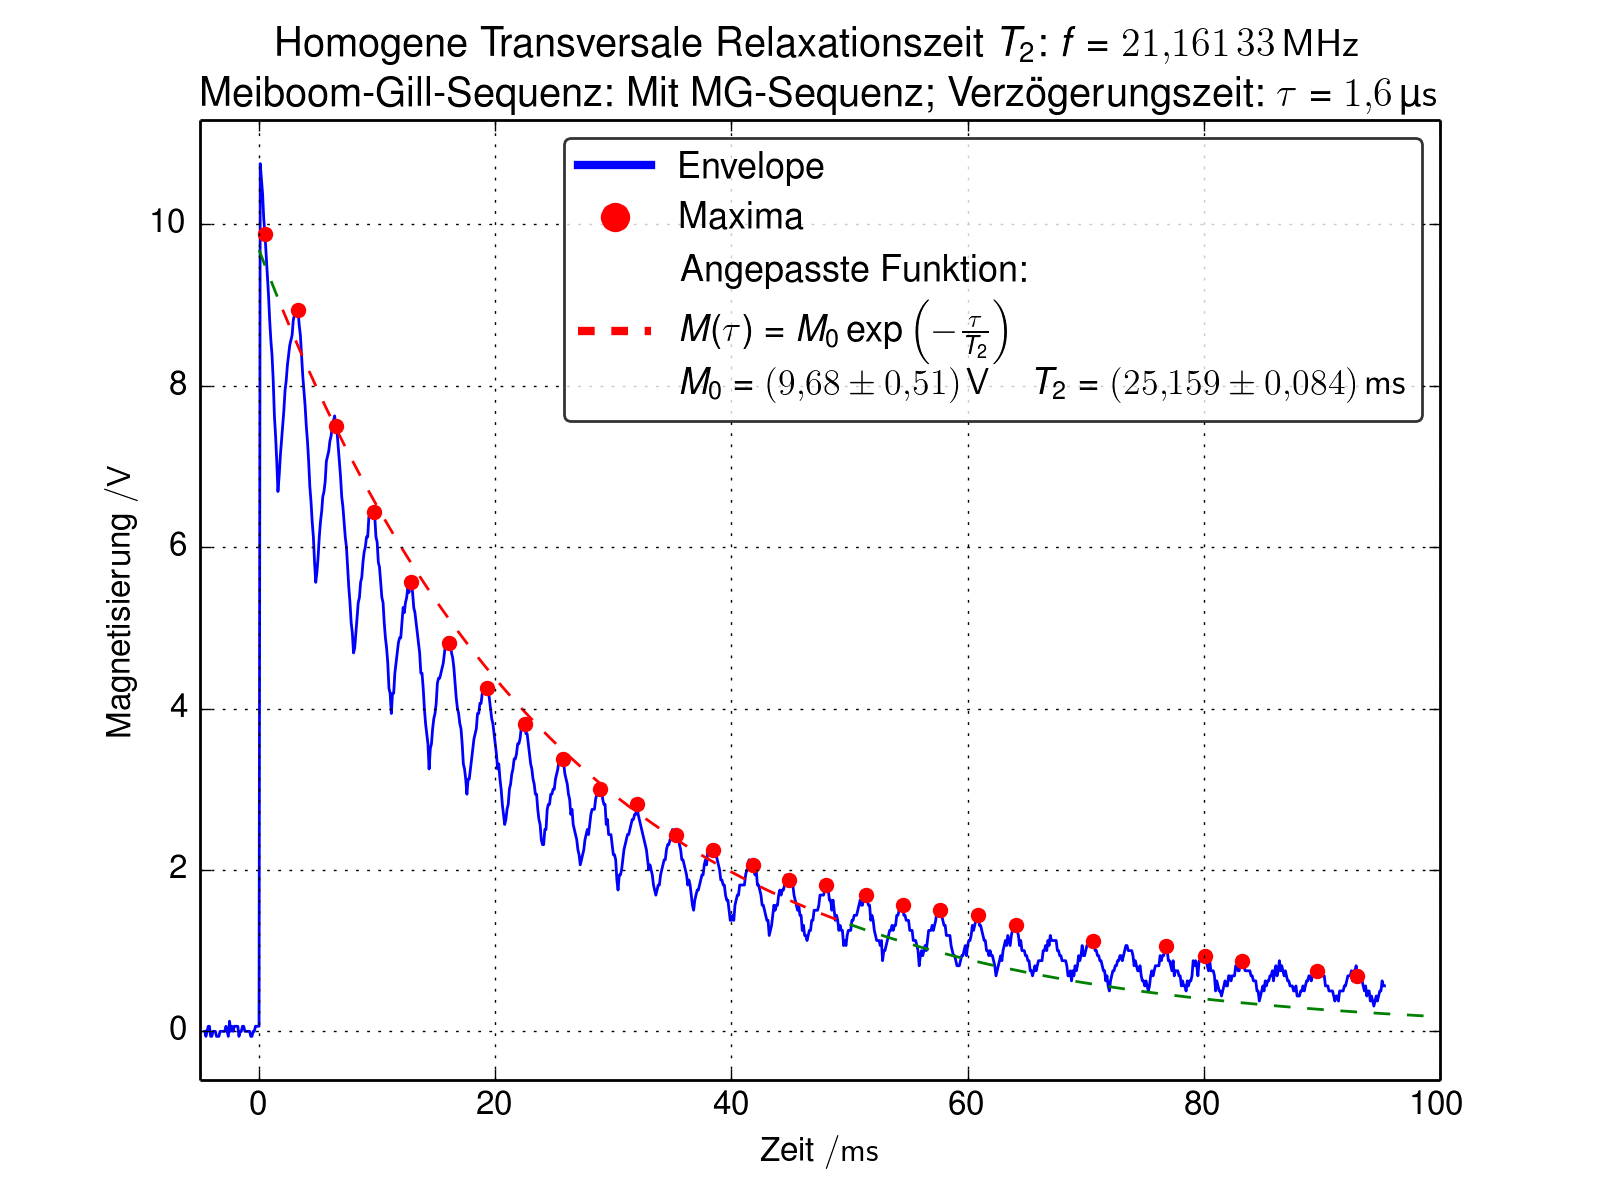
\includegraphics[width=\textwidth]
            {Figures/HomoTransRelax_MG_env1.png}
            \caption{Verlauf der lokalen Maxima des Antwort - Signales für die
              Meiboom--Gill - Sequenz bei $\tau = \SI{1.6}{\micro\second}$.}
            \label{figMG_env1}
          \end{minipage} \\
          \begin{minipage}{.48\textwidth}
            \centering
            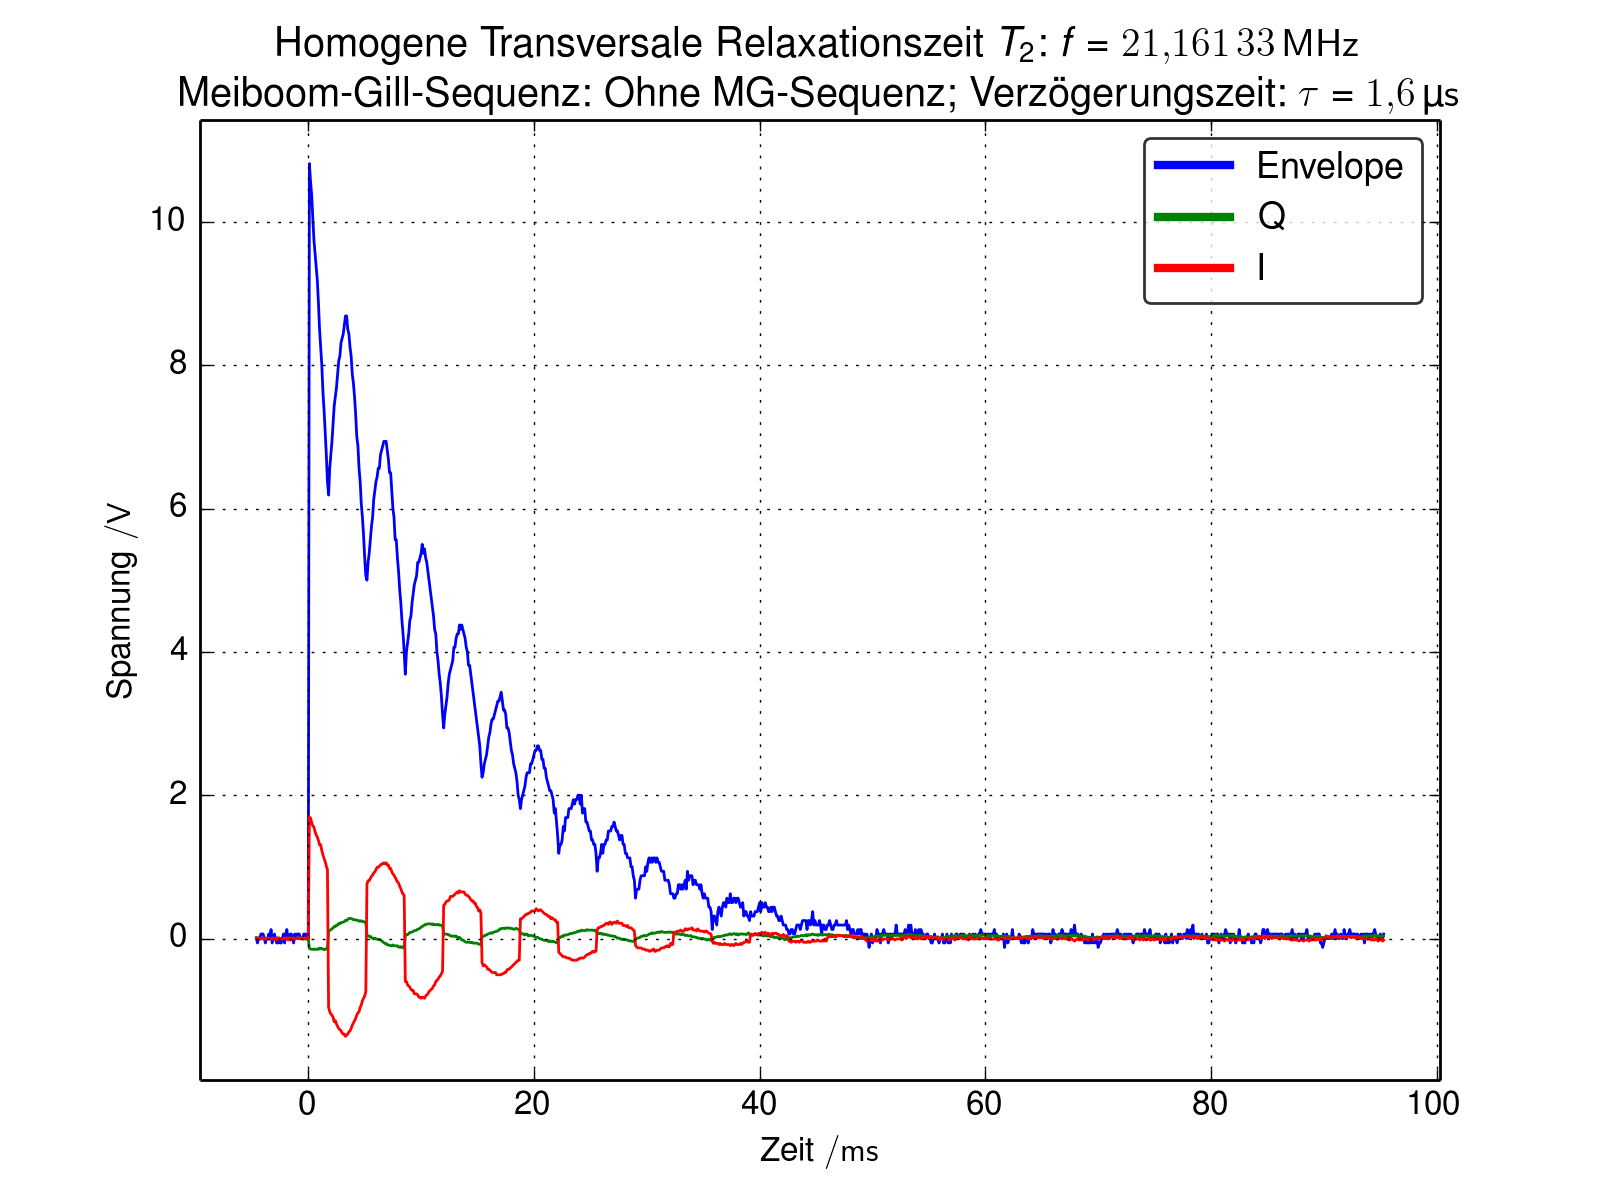
\includegraphics[width=\textwidth]
            {Figures/HomoTransRelax_MG_env_Q_I0.png}
            \caption{Spannungen des Antwort-, Q- und
              In--Phase - Signales bei der Carr--Purcell - Sequenz.}
            \label{figMG_envQI0}
          \end{minipage}\quad
          \begin{minipage}{.48\textwidth}
            \centering
            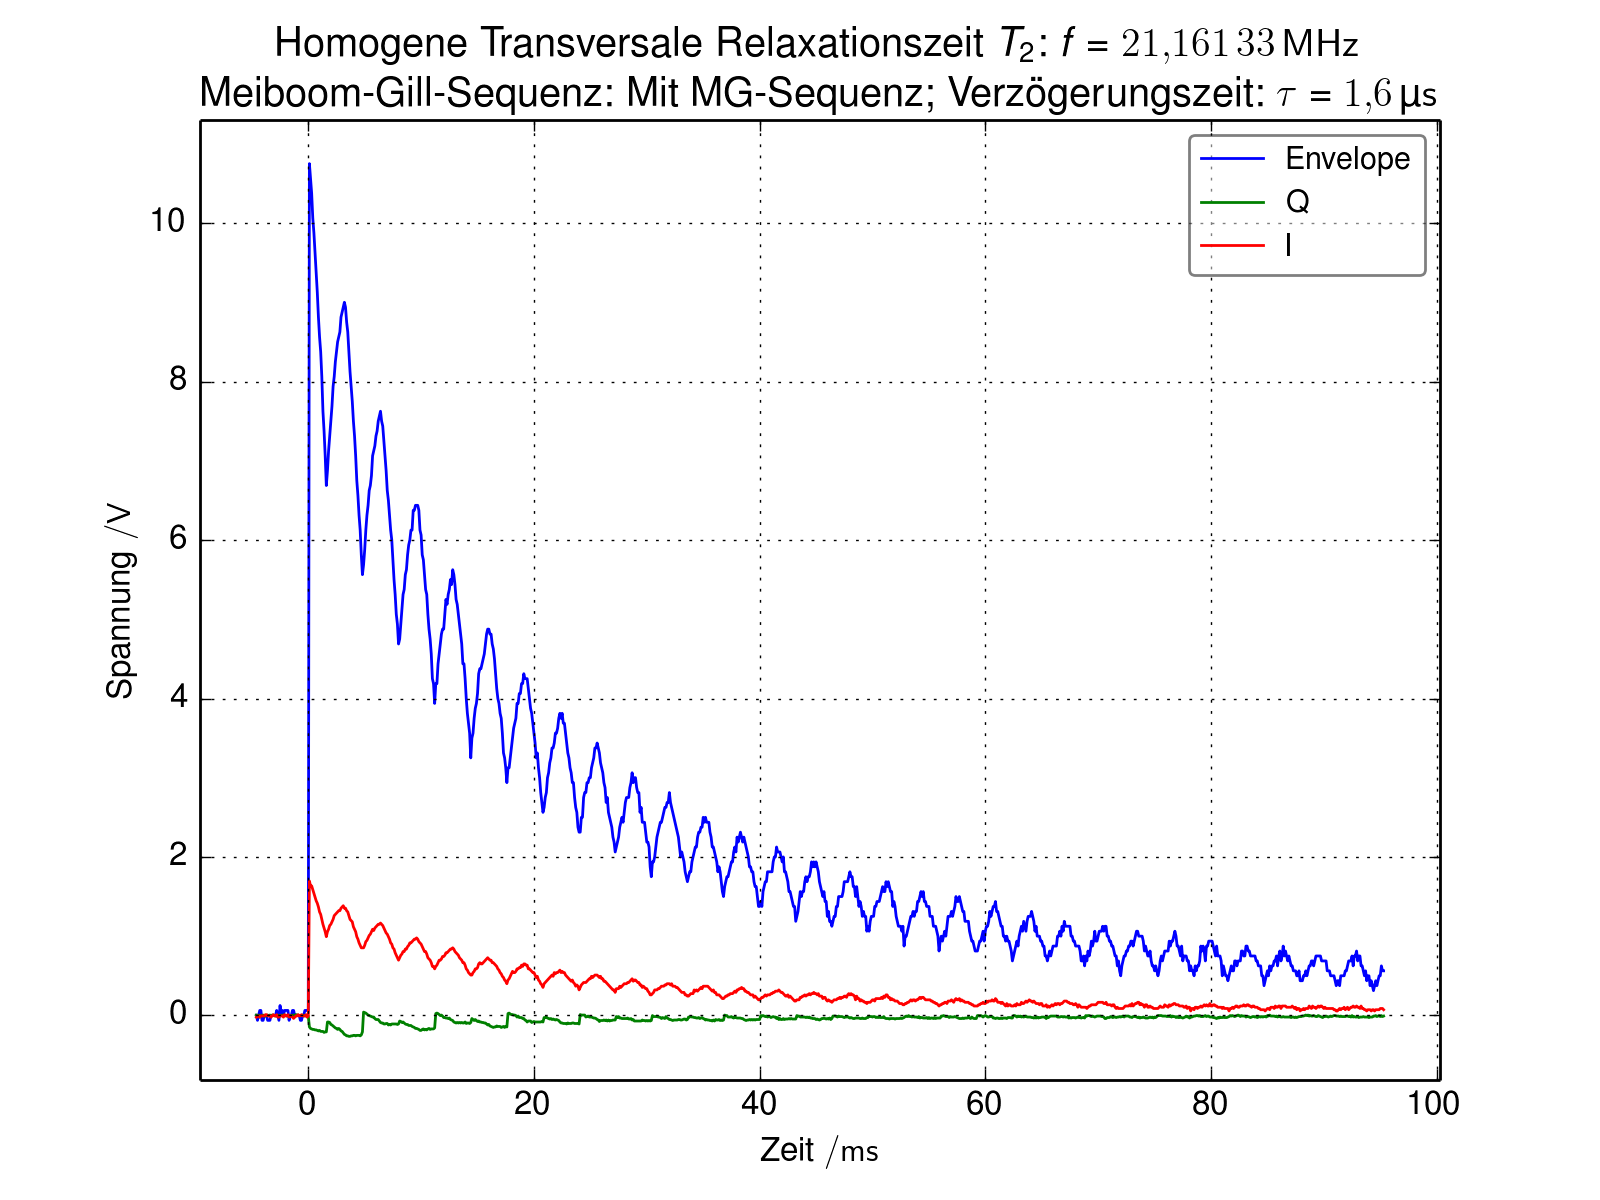
\includegraphics[width=\textwidth]
            {Figures/HomoTransRelax_MG_env_Q_I1.png}
            \caption{Spannungen des Antwort-, Q- und
              In--Phase - Signales bei der Meiboom--Gill - Sequenz.}
            \label{figMG_envQI1}
          \end{minipage}
        \end{figure}
        \todo[inline]{Beobachtung der unteren Bilder noch erklären.
          Wieso oszilliert es nicht mehr?}
        
      \end{subsection}
      %%%%%%%%%%%%%%%%%%%%%%%%%%%%%%%%%%%%%%%
      
    \end{section}
    %%%%%%%%%%%%%%%%%%%%%%%%%%%%%
    
    
    
    \newpage
    %%%%%%%%%%%%%%%%%%%%%%%%%%%%%
    %%%%%%%%%%%%%%%%%%%%%%%%%%%%%
    %%%%%%%%%%%%%%%%%%%%%%%%%%%%%
    \begin{section}{Zusammenfassung und Diskussion der Ergebnisse}
      \label{chpAuswertungDiskussion}
      
      
      %%%%%%%%%%%%%%%%%%%%%%%%%%%%%%%%%%%%%%%
      %%%%%%%%%%%%%%%%%%%%%%%%%%%%%%%%%%%%%%%
      %%%%%%%%%%%%%%%%%%%%%%%%%%%%%%%%%%%%%%%
      \begin{subsection}[Longitudinale Relaxationszeit]
        {Longitudinale Relaxationszeit $T_{1}$}
        \label{chpAuswertungDiskussionLong}
        
        
      \end{subsection}
      %%%%%%%%%%%%%%%%%%%%%%%%%%%%%%%%%%%%%%%
      
      
      
      %%%%%%%%%%%%%%%%%%%%%%%%%%%%%%%%%%%%%%%
      %%%%%%%%%%%%%%%%%%%%%%%%%%%%%%%%%%%%%%%
      %%%%%%%%%%%%%%%%%%%%%%%%%%%%%%%%%%%%%%%
      \begin{subsection}[Transversale Relaxationszeit]
        {Transversale Relaxationszeit $T_{2}$}
        \label{chpAuswertungDiskussionTrans}
        
        
      \end{subsection}
      %%%%%%%%%%%%%%%%%%%%%%%%%%%%%%%%%%%%%%%
      
    \end{section}
    %%%%%%%%%%%%%%%%%%%%%%%%%%%%%
   
  \end{chapter}
  %%%%%%%%%%%%%%%%%%%%
  
  
  
  %%%%%%%%%%%%%%%%%%%%
  %%%%%%%%%%%%%%%%%%%%
  %%%%%%%%%%%%%%%%%%%%
  %%%%%%%%%%%%%%%%%%%%
%%%%%%%%%%%%%%%%%%%%
%%%%%%%%%%%%%%%%%%%%
\begin{appendix}
  \label{Anhang}
  
  
  
  %%%%%%%%%%%%%%%%%%%%%%%%%%%%%%
  %%%%%%%%%%%%%%%%%%%%%%%%%%%%%%
  %%%%%%%%%%%%%%%%%%%%%%%%%%%%%%
  \begin{chapter}{ERSTER TEIL}
    \label{Anhang:chp:ERSTERTEIL}
    
    
    
  \end{chapter}
  %%%%%%%%%%%%%%%%%%%%%%%%%%%%%%
  
  
  
  %%%%%%%%%%%%%%%%%%%%%%%%%%%%%%
  %%%%%%%%%%%%%%%%%%%%%%%%%%%%%%
  %%%%%%%%%%%%%%%%%%%%%%%%%%%%%%
  \begin{chapter}{ZWEITER TEIL}
    \label{Anhang:chp:ZWEITERTEIL}
    
    
    
  \end{chapter}
  %%%%%%%%%%%%%%%%%%%%%%%%%%%%%%
  
\end{appendix}
%%%%%%%%%%%%%%%%%%%%
 
  %%%%%%%%%%%%%%%%%%%%
  
  
  
  %%%%%%%%%%%%%%%%%%%%
  %%%%%%%%%%%%%%%%%%%%
  %%%%%%%%%%%%%%%%%%%%
  \begin{thebibliography}{99}
    \scriptsize
    \bibitem{bib:Anleitung}\url{http://www.praktika.physik.uni-bonn.de/module/physik412/downloads/p441d}
\bibitem{bib:}\url{bla}
  \end{thebibliography}
  %%%%%%%%%%%%%%%%%%%%
 
\end{document}
%%%%%%%%%%
